\addchap{Anhang A - Planung}
\setcounter{chapter}{1}
\setcounter{section}{0}
\setcounter{table}{0}
\setcounter{figure}{0}
%
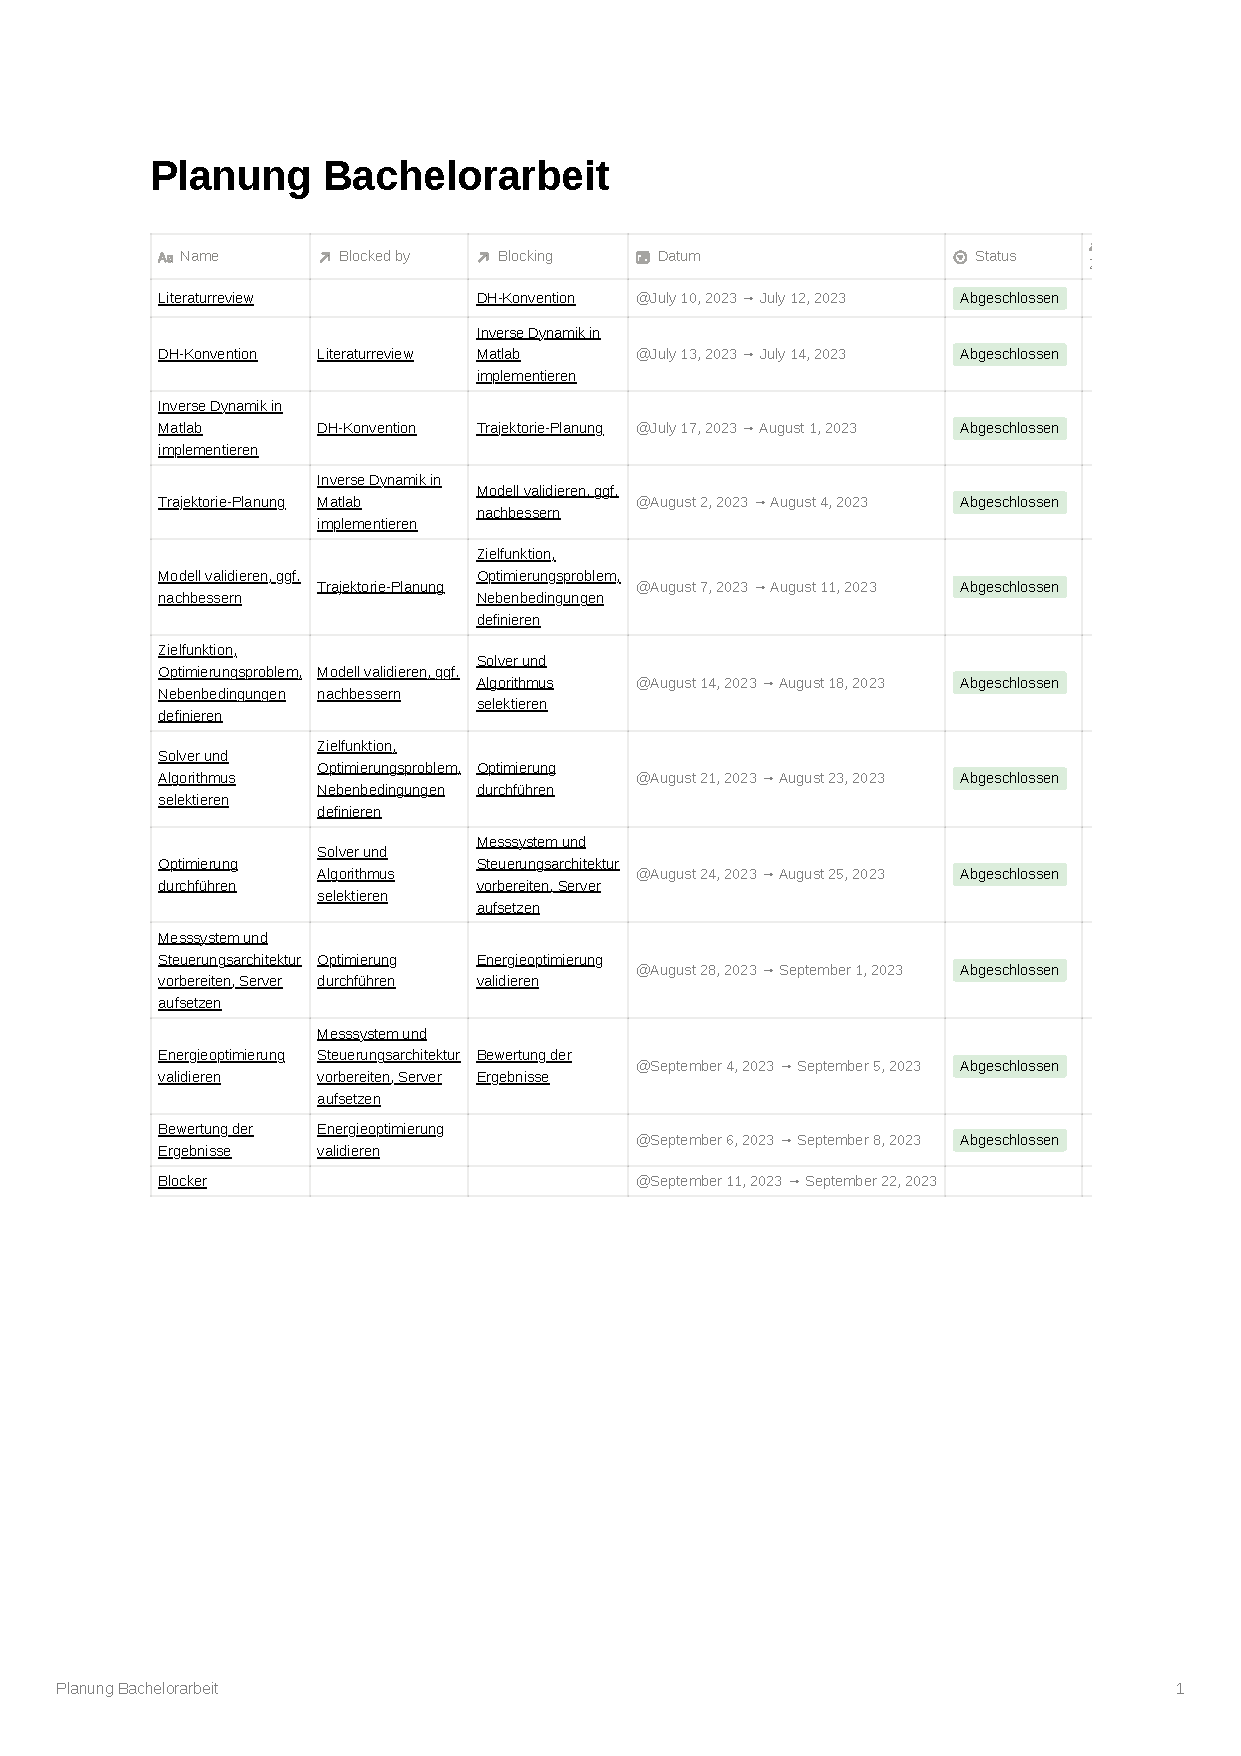
\includepdf[pages=1]{C:/Users/denni/Documents/Bachelorarbeit/BachelorThesis/literature/Anhang/planung.pdf}
\label{add:PSP}




\addchap{Anhang B - Theoretische Grundlagen}
\setcounter{chapter}{2}
\setcounter{section}{0}
\setcounter{table}{0}
\setcounter{figure}{0}
%
\section{Kinematische Kette}
\label{add:kinematische-kette}
Als kinematische Kette wird die Zusammensetzung eines Roboterarms aus $n+1$ Gliedern und $n$ Gelenken definiert. Das letzte Glied der kinematischen Kette wird als Endeffektor bezeichnet. Die Glieder werden von der festen Basis (Glied $0$) bis $n$ durchnummeriert. Mit jedem Glied $i-1$ wird das Gelenk $i$ starr verbunden. Des Weiteren wird jedem Glied $i$ ein fest verbundenes Koordinatensystem $o_ix_iy_iz_i$ zugeordnet. Eine Aktuierung des Gelenks $i$ führt zu einer Bewegung von Glied $i$ und Koordinatensystem KS$\left\{i\right\}$. Die Gelenke weisen einen Freiheitsgrad (degree-of-freedom (DOF)) $q_i$ auf und können als Dreh- oder Schubgelenke ausgeführt werden. Die Gelenkvariable $q_i$ entspricht dem Rotationswinkel $\theta_i$ bzw. der Translation $d_i$. \cite[S.~75]{Spong.2020}
%
\setcounter{section}{1}
\section{Euklidische Gruppe}
\label{add:SE3}
\begin{align} 
	\text{SE(3)} = \left\{{\bm{T}} \ | \ \bm{T}=\begin{bmatrix} {\bm{R}} &\quad {\bm{o}}\\ \bm{0}_{1x3} &\quad 1 \end{bmatrix}\right\}, \ \bm{R} \in {R}^{3x3}, \ {r} \in {R}^{3}  
\end{align} 

\cite[S.~534]{Spong.2020}
\setcounter{section}{2}
\section{Geschwindigkeits-Kinematik}
\label{add:geschwindigkeitskinematik}
Die Herleitung der Zusammenhänge ist  \cite[S.~79~f.]{Kemmetmueller.2023} und  \cite[S.~106]{Spong.2020} entnommen. Die Rotation eines Starrk{\"o}rpers um eine feste Drehachse wird über die Beziehung $\bm{\omega} = \dot{\theta}\bm{k}$ ausgedr{\"u}ckt. Dabei sind $\dot{\theta}$ die zeitliche Ableitung des Gelenkwinkels $\theta$ und $\bm{k}$ der Einheitsvektor der Drehachse. Die lineare Geschwindigkeit eines Punktes P, welcher um die Drehachse rotiert, ergibt sich zu $\bm{v} = \bm{\omega} \times \bm{r}$. Wobei der Vektor $\bm{r}$ die Position des Punktes P orthogonal auf der Drehachse $\bm{k}$ angibt. \cite[S.~102]{Spong.2020} 
%
\subsection{Schiefsymmetrische Matrizen}
Die Berechnung der Geschwindigkeits-Kinematik l{\"a}sst sich durch Verwendung Schiefsymmetrischer Matrizen vereinfachen. Eine $n\times n$ Matrix $\bm{S}$ ist schief symmetrisch, wenn 
\begin{equation}
	\label{eqn:skewsymmetric}
	\bm{S}^T+\bm{S}=0.
\end{equation}
Damit hat jede schiefsymmetrische $3\times3$ Matrix die Form
\begin{align}
	\bm{S} = \left[\begin{matrix}
		0 &\quad -s_3 &\quad s_2  \\
		s_3 &\quad 0 &\quad -s_1  \\
		-s_2 &\quad s_1 &\quad 0  
	\end{matrix}\right].
\end{align}
Für weitere Eigenschaften schiefsymmetrischer Matrizen wird auf die referenzierte Literatur \cite[S.~104]{Spong.2020} verwiesen. Für die Drehmatrix $\bm{R} = \bm{R}(\theta) \in SO(3)$, deren Elemente Funktionen der Drehwinkel $\theta\left(t\right)$ sind, gilt 
\begin{equation}
	\label{eqn:einheitsmatrix}
	\bm{R}(\theta)\bm{R}(\theta)^T = \bm{E}.
\end{equation}
%
\subsection{Drehwinkelgeschwindigkeit}
Die Ableitung beider Terme der Gleichung \ref{eqn:einheitsmatrix} ergibt
\begin{equation} 
	\dfrac{\text{d}}{\text{d}\theta}\left[\bm{R}(\theta)\bm{R}(\theta)^T\right] = 	\left[\dfrac{\text{d}}{\text{d}\theta} {\bm{R}}(\theta)\right]\bm{R}(\theta)^T + \bm{R}(\theta)\left[\dfrac{\text{d}}{\text{d}\theta} {\bm{R}}(\theta)^T\right] = 0
\end{equation} 
Unter Berücksichtigung der Eigenschaft schiefsymmetrischer Matrizen, siehe Gleichung \ref{eqn:skewsymmetric} folgt
\begin{equation}
	\label{eqn:skewsymm}
	\bm{S} = \left[\dfrac{\text{d}}{\text{d}\theta}{\bm{R}}(\theta)\right]\bm{R}(\theta)^T  = -\bm{R}(\theta)     \left[\dfrac{\text{d}}{\text{d}\theta}{\bm{R}}(\theta)^T\right].
\end{equation} 
%
Daraus folgt
%
\begin{equation}
	\dfrac{\text{d}}{\text{d}\theta}\bm{R}(\theta) = \bm{SR}(\theta)
\end{equation} 
%
Die zeitliche Ableitung der Rotationsmatrix $\bm{R} = \bm{R}(t) \in SO(3)$ lautet
%
\begin{equation}
	\dfrac{\text{d}}{\text{d}t}\bm{R}(t) = \bm{S}\left(\bm{\omega}(t)\right)\bm{R}(t)
\end{equation} 
%
Für Verkettete Rotationen gilt
%
\begin{equation}
	\dfrac{\text{d}}{\text{d}t}\bm{R}^0_n(t) = \bm{S}\left(\bm{\omega}^0_{0,n}(t)\right)\bm{R}^0_n(t)
\end{equation} 
\begin{equation}
	\bm{\omega}^0_{0,n} = \bm{\omega}^0_{0,1} + \bm{R}^0_1\bm{\omega}^1_{1,2} + \bm{R}^0_2\bm{\omega}^2_{2,3} + ... + \bm{R}^0_{n-1}\bm{\omega}^{n-1}_{n-1,n}
\end{equation} 
%
%Die Elemente von $\bm{S}$ resultieren aus den Winkelgeschwindigkeiten $\omega = \left[\omega_x~\omega_y~\omega_z\right]^T$.
%\begin{equation}
%	\bm{S} = \left[\begin{array}{ccc}
	%		0&-\omega_z&\omega_y  \\
	%		\omega_z&0&-\omega_x  \\
	%		-\omega_y&\omega_x&0  \\
	%	\end{array} \right]
%\end{equation}
%
\subsection{Lineare Geschwindigkeit}
Für die Lineare Geschwindigkeit eines Punktes werden nachfolgend zwei Szenarien unterschieden. In beiden Fällen ist der Punkt P fest mit dem KS$\left\{i\right\}$ verbunden. Im ersten Fall wird eine Rotation des KS$\left\{i\right\}$ relativ zum KS$\left\{0\right\}$ betrachtet. 
\begin{equation}
	\bm{p}^0 = \bm{R}^0_i(t)\bm{p}^i
\end{equation}
%
\begin{equation}
	\dot{\bm{p}}^0 = \bm{\omega}^0_{0,i}\times\bm{p}^0
\end{equation}
%
Im zweiten Fall bewegt sich KS$\left\{i\right\}$ rotatorisch und translatorisch relativ zu KS$\left\{0\right\}$. 
\begin{equation}
	\bm{p}^0 = \bm{R}^0_i(t)\bm{p}^i + \bm{o^0_i}
\end{equation}
%
\begin{equation}
	\dot{\bm{p}}^0 = \bm{\omega}^0_{0,i}\times\bm{p}^0 + \dot{\bm{o^0_i}}
\end{equation}
Auf eine Beschreibung des Szenarios, dass sich P gegenüber KS$\left\{i\right\}$ bewegt, wird verzichtet.
%
\subsection*{Jacobi-Matrizen}
Die lineare Geschwindigkeit $\bm{v}^0_n$ des Endeffektors, sowie seine Winkelgeschwindigkeit $\bm{\omega}^0_{0,n}$ ausgedrückt in KS$\left\{0\right\}$ lassen sich über die $3\times n$-Jacobi-Matrizen $\bm{J}_v$ und $\bm{J}_{\omega}$ berechnen. 
%
\begin{equation}
	\bm{v}^0_n = \bm{J}_v \dot{\bm{q}} = \left[\bm{J}_{v_1} \ \bm{J}_{v_2} \ ...\  \bm{J}_{v_n}\right] \dot{\bm{q}}
\end{equation}
%
\begin{equation}
	\bm{\omega}^0_{0,i} = \bm{J}_{\omega} \dot{\bm{q}}  = \left[\bm{J}_{\omega_1} \ \bm{J}_{\omega_2} \ ...\  \bm{J}_{\omega_n}\right] \dot{\bm{q}}
\end{equation}
%
\begin{equation}
	\bm{J}_{vi} = \begin{cases} 
		\bm{z}^0_{i-1} \times (\bm{o}^0_{n} - \bm{o}^0_{i-1}) & \text{falls Gelenk } i \text{ vom Typ } \text{R} \\
		\bm{z}^0_{i-1} & \text{falls Gelenk } i \text{ vom Typ } \text{T}
	\end{cases}
\end{equation}
%
\begin{equation}
	\bm{J}_{\omega i} = \begin{cases} 
		\bm{z}^0_{i-1} = \bm{R}^0_{i-1}\bm{e}_3 & \text{falls Gelenk } i \text{ vom Typ } \text{R} \\
		\mathbf{0}_{3 \times 1} & \text{falls Gelenk } i \text{ vom Typ } \text{T}
	\end{cases}
\end{equation}
%
\begin{itemize}
	\item Ein Gelenk vom Typ R ist ein Rotationsgelenk.
	\item Ein Gelenk vom Typ T ist ein Translationsgelenk.
\end{itemize}
%
\cite{Rieber.2022}
%
%\section{Newtonsche Axiome} 
%\section{Zwangsbedingungen}
%	- %todo holonom
%	Holonome Zwangsbedingungen sind als Gleichungen formulierbar
%	drei Positionskoordinaten definieren die Lage des Massenschwerpunkts eines Arms
%	drei Eulerwinkel definieren die Orientierung des Körpers
%	- %todo nicht holomom
%	Nichtholonome Zwansbedingungen sind nicht als Gleichungen formulierbar, z. B. Ungleichungen
%\section{Hamilton-Prinzip}
%\section{D’Alembertsches Prinzip}
%\section{Weitere Details, welche im Hauptteil den Lesefluss behindern}
%
%\addchap{Anhang B}
%\setcounter{chapter}{2}
%\setcounter{section}{0}
%\setcounter{table}{0}
%\setcounter{figure}{0}
%
%\section{Versuchsanordnung}
%
%\section{Liste der verwendeten Messgeräte}
%
%\section{Übersicht der Messergebnisse}
%
%\section{Schaltplan und Bild der Prototypenplatine}

%\clearpage
%
%Diese Seite wurde eingefügt, um zu zeigen, wie sich der Inhalt der Kopfzeile automatisch füllt.
%
%\addchap{Anhang C}
%\setcounter{chapter}{3}
%\setcounter{section}{0}
%\setcounter{table}{0}
%\setcounter{figure}{0}
%
%\section{Struktogramm des Programmentwurfs}
%
%\section{Wichtige Teile des Quellcodes}
%
\addchap{Anhang B - Roboterdaten}
\setcounter{chapter}{3}
\setcounter{section}{0}
\setcounter{table}{0}
\setcounter{figure}{0}
%
%\section{Einbinden von PDF-Seiten aus anderen Dokumenten}
%
%Auf den folgenden Seiten wird eine Möglichkeit gezeigt, wie aus einem anderen PDF-Dokument komplette Seiten übernommen werden können. Der Nachteil dieser Methode besteht darin, dass sämtliche Formateinstellungen (Kopfzeilen, Seitenzahlen, Ränder, etc.) auf diesen Seiten nicht angezeigt werden. Die Methode wird deshalb eher selten gewählt. Immerhin sorgt das Package \textit{\glqq pdfpages\grqq}~für eine korrekte Seitenzahleinstellung auf den im Anschluss folgenden \glqq nativen\grqq~\LaTeX-Seiten.
%
%Eine bessere Alternative ist, einzelne Seiten mit \textit{\glqq$\backslash$includegraphics\grqq}~einzubinden. Z.B. wenn Inhalte von Datenblättern wiedergegeben werden sollen.

\section{KR210 2700-2 Datenblatt}
\label{add:datenblatt}
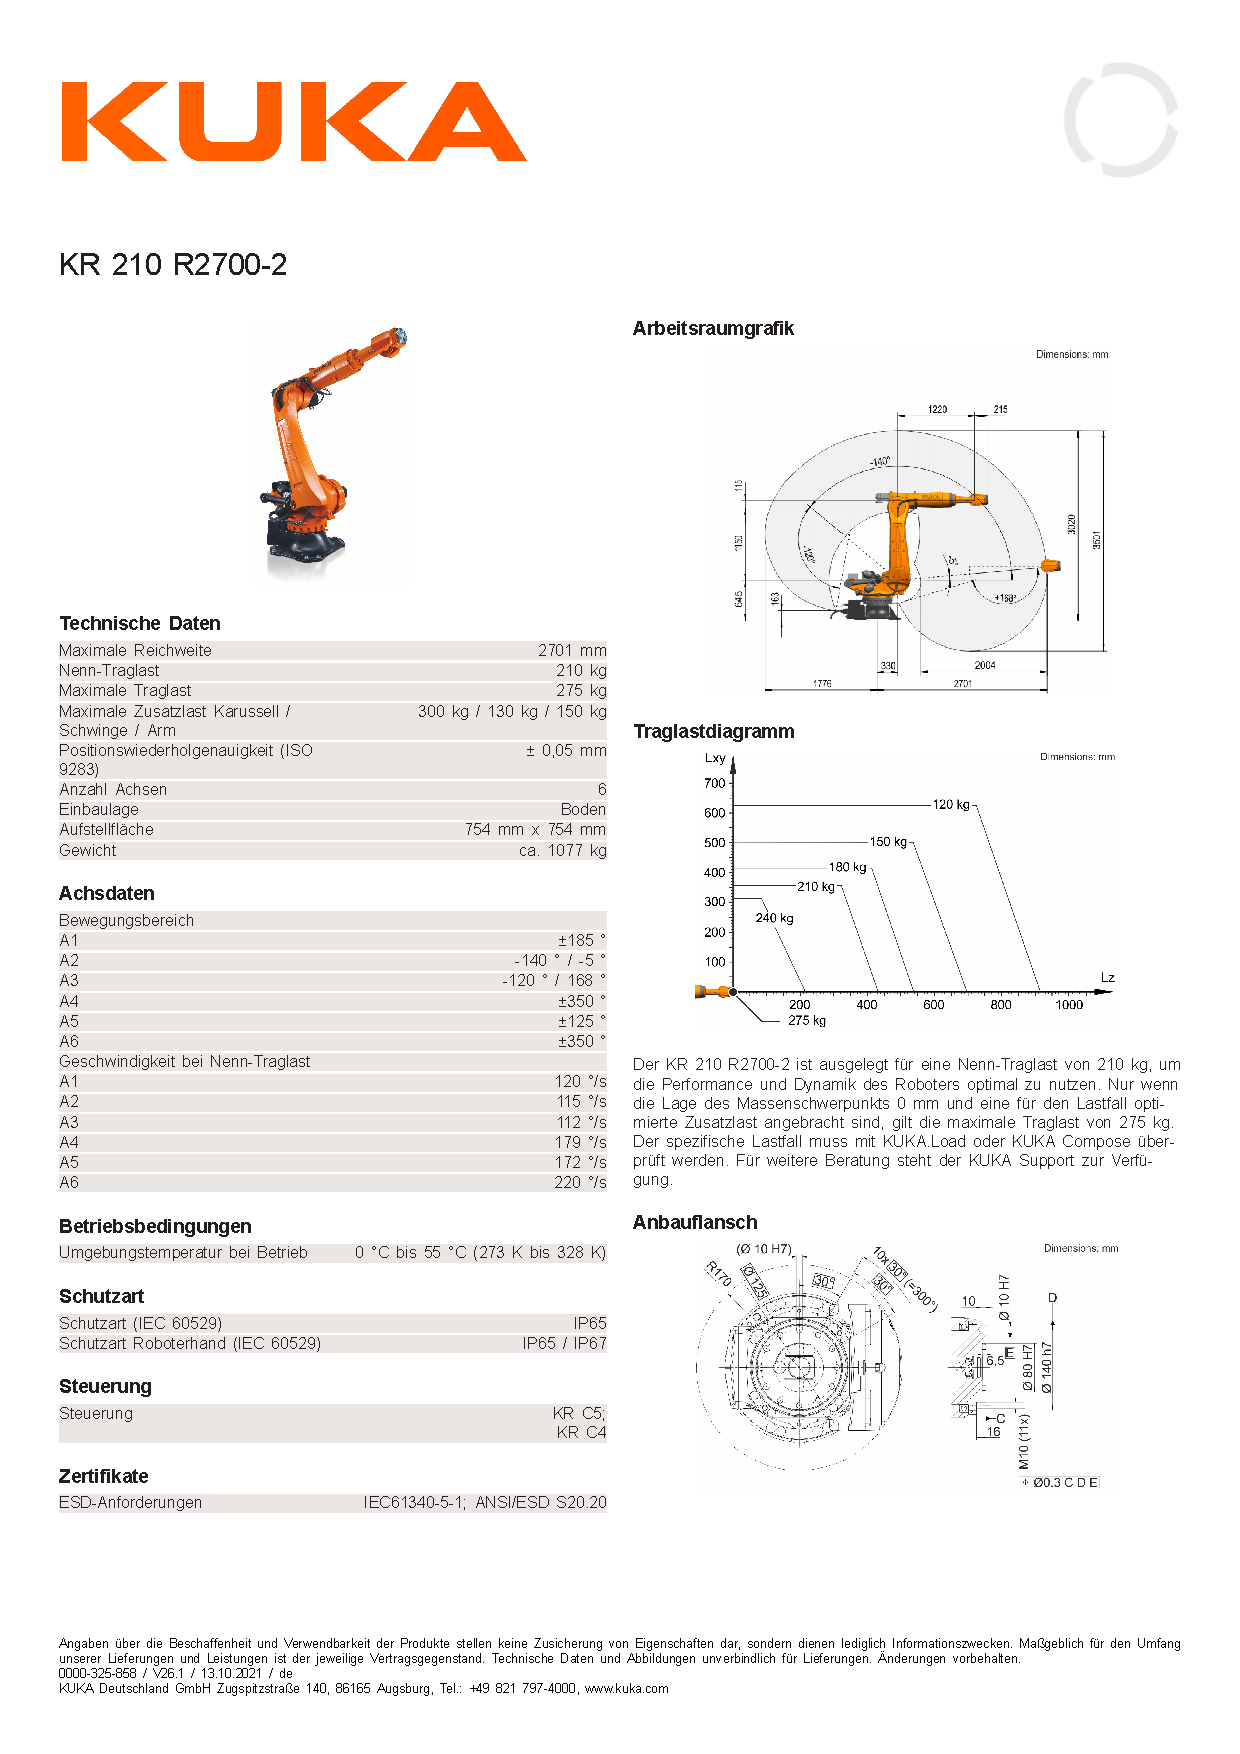
\includepdf[pages=1]{C:/Users/denni/Documents/Bachelorarbeit/BachelorThesis/literature/Anhang/DatenblattKR2102700-2.pdf}
\setcounter{section}{1}
\section{Systemparameter}
\label{add:Systemparameterdef}
Die Massen $m_i$ der Starrkörper $i$, siehe Tabelle \ref{tab:masse} sind dem CAD-Modell des Herstellers entnommen. Hierbei wird angenommen, dass der Werkstoff korrekt zugeordnet ist. 

\begin{table}[hptb]
	\centering
	\caption{Massen der Verbindungsglieder in $\left[\mathrm{kg}\right]$}
	\label{tab:masse}
	\begin{tabular}{|c|c|c|c|c|c|}
		\hline
		$m_1$ = 535 & $m_2$ = 696,3   &$m_3$ = 361,6   & $m_4$ = 39,676 &$m_5$ = 53,619   &$m_6$ = 4,528  \\
		\hline
	\end{tabular}
\end{table}

Die Trägheitstensoren, werden vom CAD-Modell, bezogen auf das KS$\left\{0\right\}$ vorgegeben. Gleichung \ref{eqn:similarity} zeigt, wie diese einmalig über eine Ähnlichkeitstransformation auf das Körperfeste Koordinatensystem KS$\left\{i\right\}$ transformiert werden. In der Tabelle \ref{tab:tensoren} sind die Trägheitstensoren bezogen auf das KS$\left\{0\right\}$ angegeben. 

\begin{table}[hptb]
	\centering
	\caption{Trägheitstensoren in $\left[\dfrac{\text{kg}}{\text{m}^2}\right] $}
	\label{tab:tensoren}
\begin{tabular}{|l|l|l|l|l|l|}
	\hline
	$I_{1xx} = 17,3$&  $I_{2xx} = 138,14$&  $I_{3xx} = 3,03$&  $I_{4xx} = 0,1$&  $I_{5xx} = 0,48$&$I_{6xx} = 0,01$\\
	\hline
	$I_{1xy} = -2,71$&  $I_{2xy} = -0,01$&  $I_{3xy} = -1,39$&  $I_{4xy} = -0,03$&  $I_{5xy} = 0,12$&$I_{6xy} = 0$\\
	\hline
	$I_{1xz} = 1,67$&  $I_{2xz} = 0,39$&  $I_{3xz} = -0,05$&  $I_{4xz} = 0$&  $I_{5xz} = 0$&$I_{6xz} = 0$\\
	\hline
	$I_{1yy} = 32,67$&  $I_{2yy} = 136,66$&  $I_{3yy} = 30,03$&  $I_{4yy} = 0,7$&  $I_{5yy} = 0,42$&$I_{6yy} = 0,01$\\
	\hline
	$I_{1yz} = -0,49$&  $I_{2yz} = 9,23$&   $I_{3yz} = -0,21$&  $I_{4yz} = 0$&  $I_{5yz} = 0$&$I_{6yz} = 0$\\
	\hline
	$I_{1zz} = 29,45$&  $I_{2zz} = 11,84$&  $I_{3zz} = 29,69$&  $I_{4zz} = 0,7$&  $I_{5zz} = 0,68$&$I_{6zz} = 0,01$\\
	\hline
\end{tabular}
\end{table}
Nachfolgend ist die Lage der Massenschwerpunkte $C_i^0$ im KS$\left\{0\right\}$ angegeben. 

\begin{itemize}
	\item[] $r_{0,C_1}^0$ = $\left[-30,103,~441,~452,213\right]$ mm
	\item[] $r_{0,C_2}^0$ = $\left[330,979,~-222,585,~1094,239\right]$ mm
	\item[] $r_{0,C_3}^0$ = $\left[705,894,~-8,126,~1908,436\right]$ mm
	\item[] $r_{0,C_4}^0$ = $\left[1383,185,~4,492,~1909,983\right]$ mm
	\item[] $r_{0,C_5}^0$ = $\left[1601,767,~33,833,~1909,955\right]$ mm
	\item[] $r_{0,C_6}^0$ = $\left[1743,222,~-0,007,~1910 051\right]$ mm
\end{itemize}

Die Getriebeübersetzung in Tabelle \ref{tab:getriebe} ist der Datei Machine Data (MADA) der Robotersteuerung entnommen.

\begin{table}[hptb]
	\centering
	\caption{Getriebeübersetzung}
	\label{tab:getriebe}
\begin{tabular}{|c|c|c|c|c|c|}
	\hline
	$i_1 = -\dfrac{7}{1798}$& $i_2 = -\dfrac{17}{4576}$  &$i_3 = \dfrac{3}{754}$  & $i_4 = -\dfrac{55}{10387}$ &$i_5 = -\dfrac{483}{91834}$  &$i_6 = \dfrac{49400}{6485103}$  \\
	\hline
\end{tabular}
\end{table}

\addchap{Anhang C - MATLAB-Implementierung}
\setcounter{chapter}{4}
\setcounter{section}{0}
\setcounter{table}{0}
\setcounter{figure}{0}
\section{DH-Transformation}
\label{add:dh}
%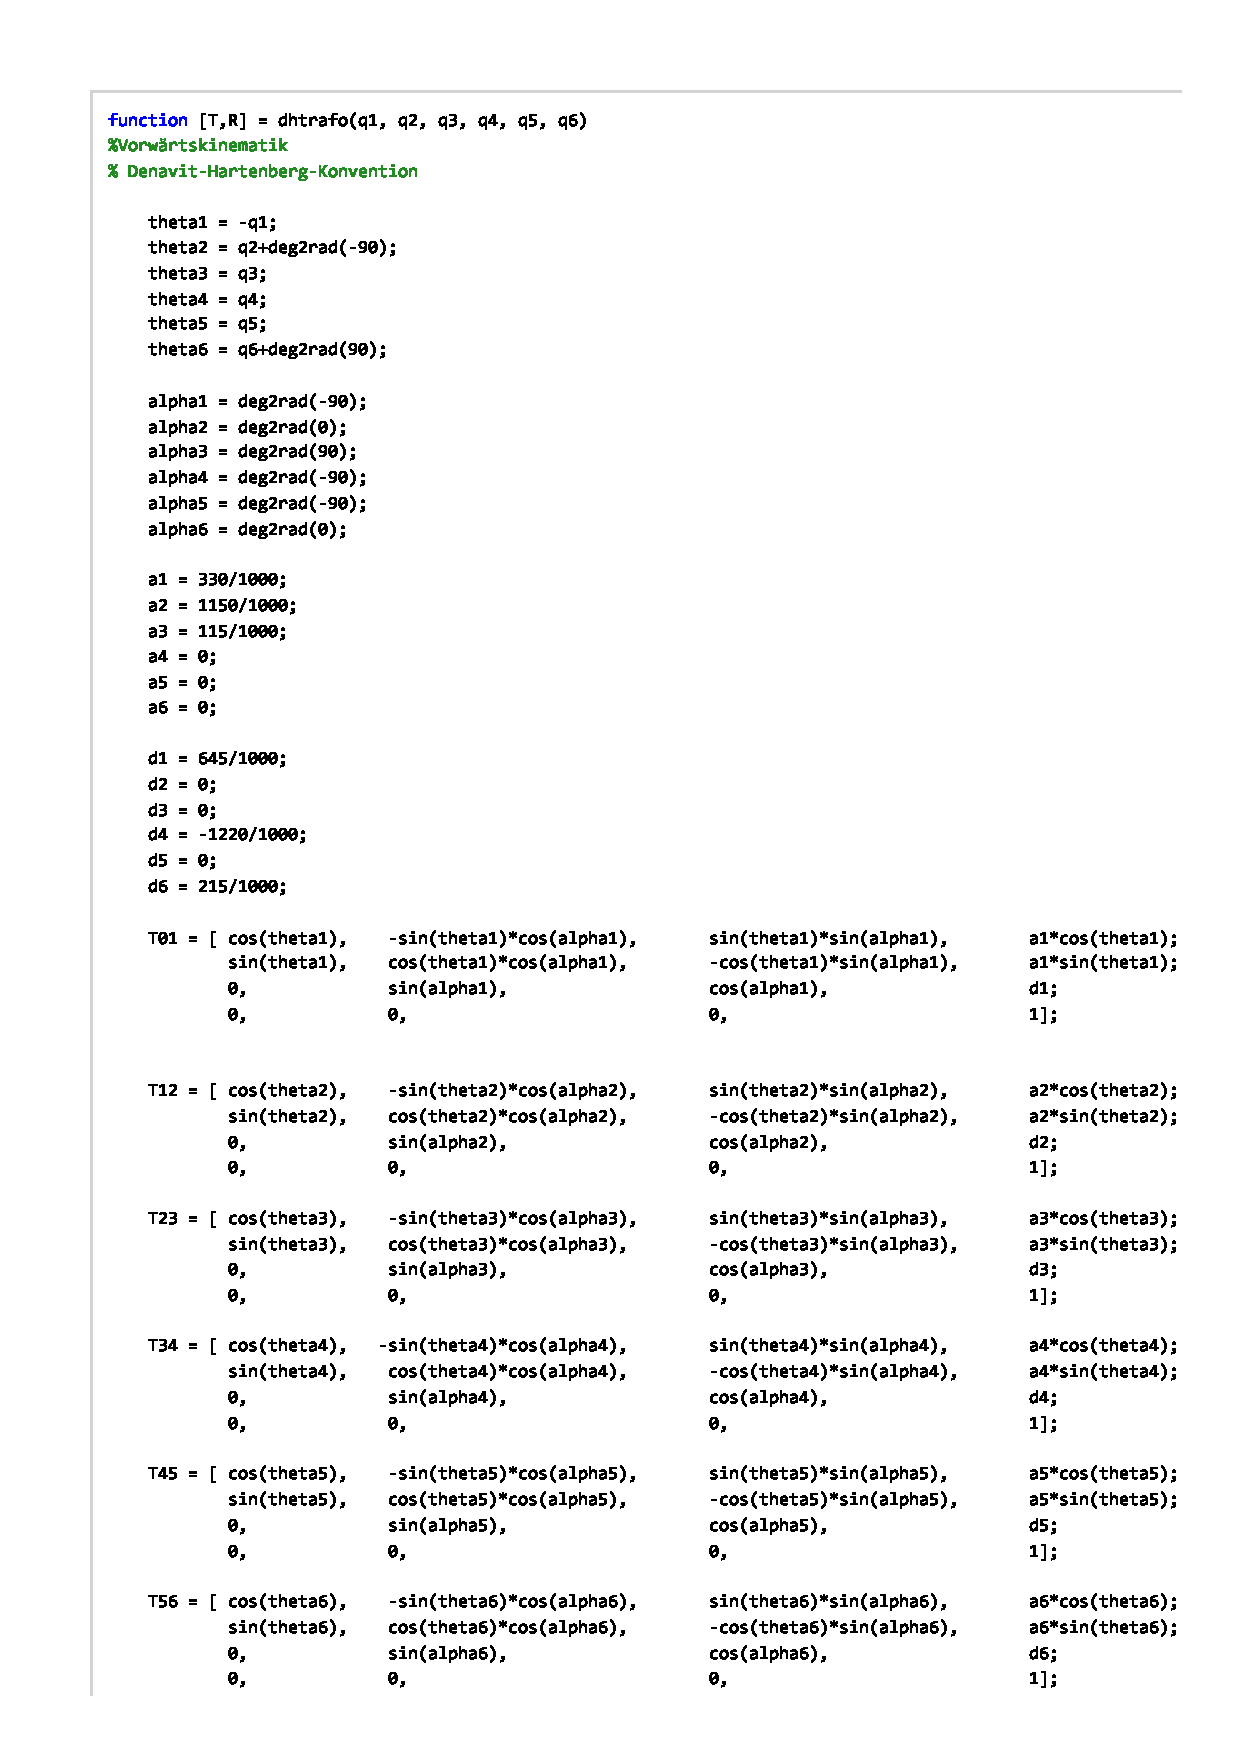
\includepdf[pages=1-2]{C:/Users/denni/Documents/Bachelorarbeit/BachelorThesis/literature/Anhang/dhtrafo_matlab.pdf}
\begin{lstlisting}[language=Matlab, numbers=none]
function [T,R,R0i] = dhtrafo(q1, q2, q3, q4, q5, q6)
%Vorwärtskinematik
% Denavit-Hartenberg-Konvention

theta1 = -q1;
theta2 = q2+deg2rad(-90);
theta3 = q3;
theta4 = q4;
theta5 = q5;
theta6 = q6+deg2rad(90);

alpha1 = deg2rad(-90);
alpha2 = deg2rad(0);
alpha3 = deg2rad(90);
alpha4 = deg2rad(-90);
alpha5 = deg2rad(-90);
alpha6 = deg2rad(0);

a1 = 330/1000;
a2 = 1150/1000;
a3 = 115/1000;
a4 = 0;
a5 = 0;
a6 = 0;

d1 = 645/1000;
d2 = 0;
d3 = 0;
d4 = -1220/1000;
d5 = 0;
d6 = 215/1000;

T01 = [ cos(theta1), -sin(theta1)*cos(alpha1), sin(theta1)*sin(alpha1), a1*cos(theta1);
		sin(theta1), cos(theta1)*cos(alpha1), -cos(theta1)*sin(alpha1), a1*sin(theta1);
		0, sin(alpha1), cos(alpha1), d1;
		0, 0, 0, 1];


T12 = [ cos(theta2), -sin(theta2)*cos(alpha2), sin(theta2)*sin(alpha2), a2*cos(theta2);
		sin(theta2), cos(theta2)*cos(alpha2), -cos(theta2)*sin(alpha2), a2*sin(theta2);
		0, sin(alpha2), cos(alpha2), d2;
		0, 0, 0, 1];

T23 = [ cos(theta3), -sin(theta3)*cos(alpha3), sin(theta3)*sin(alpha3), a3*cos(theta3);
		sin(theta3), cos(theta3)*cos(alpha3), -cos(theta3)*sin(alpha3), a3*sin(theta3);
		0, sin(alpha3), cos(alpha3), d3;
		0, 0, 0, 1];

T34 = [ cos(theta4), -sin(theta4)*cos(alpha4), sin(theta4)*sin(alpha4), a4*cos(theta4);
		sin(theta4), cos(theta4)*cos(alpha4), -cos(theta4)*sin(alpha4), a4*sin(theta4);
		0, sin(alpha4), 
	 cos(alpha4), d4;
		0, 0, 0, 1];

T45 = [ cos(theta5), -sin(theta5)*cos(alpha5), sin(theta5)*sin(alpha5), a5*cos(theta5);
		sin(theta5), cos(theta5)*cos(alpha5), -cos(theta5)*sin(alpha5), a5*sin(theta5);
		0, sin(alpha5), cos(alpha5), d5;
		0, 0, 0, 1];

T56 = [ cos(theta6), -sin(theta6)*cos(alpha6), sin(theta6)*sin(alpha6), a6*cos(theta6);
		sin(theta6), cos(theta6)*cos(alpha6), -cos(theta6)*sin(alpha6), a6*sin(theta6);
		0, sin(alpha6), cos(alpha6), d6;
		0, 0, 0, 1];

T = cat(3, T01, T12, T23, T34, T45, T56);

R01 = T01(1:3,1:3);
R12 = T12(1:3,1:3);
R23 = T23(1:3,1:3);
R34 = T34(1:3,1:3);
R45 = T45(1:3,1:3);
R56 = T56(1:3,1:3);

T02 = T01*T12;
T03 = T02*T23;
T04 = T03*T34;
T05 = T04*T45;
T06 = T05*T56;

R02 = T02(1:3,1:3);
R03 = T03(1:3,1:3);
R04 = T04(1:3,1:3);
R05 = T05(1:3,1:3);
R06 = T06(1:3,1:3);

R = cat(3, R01, R12, R23, R34, R45, R56);
R0i = cat(3, R01, R02, R03, R04, R05, R06);

end
\end{lstlisting}
\label{add:systemparameter}
%
%Nachfolgend ist die Umsetzung der Parameter Transformation via MATLAB\textsuperscript{\textregistered} gezeigt. 
%
%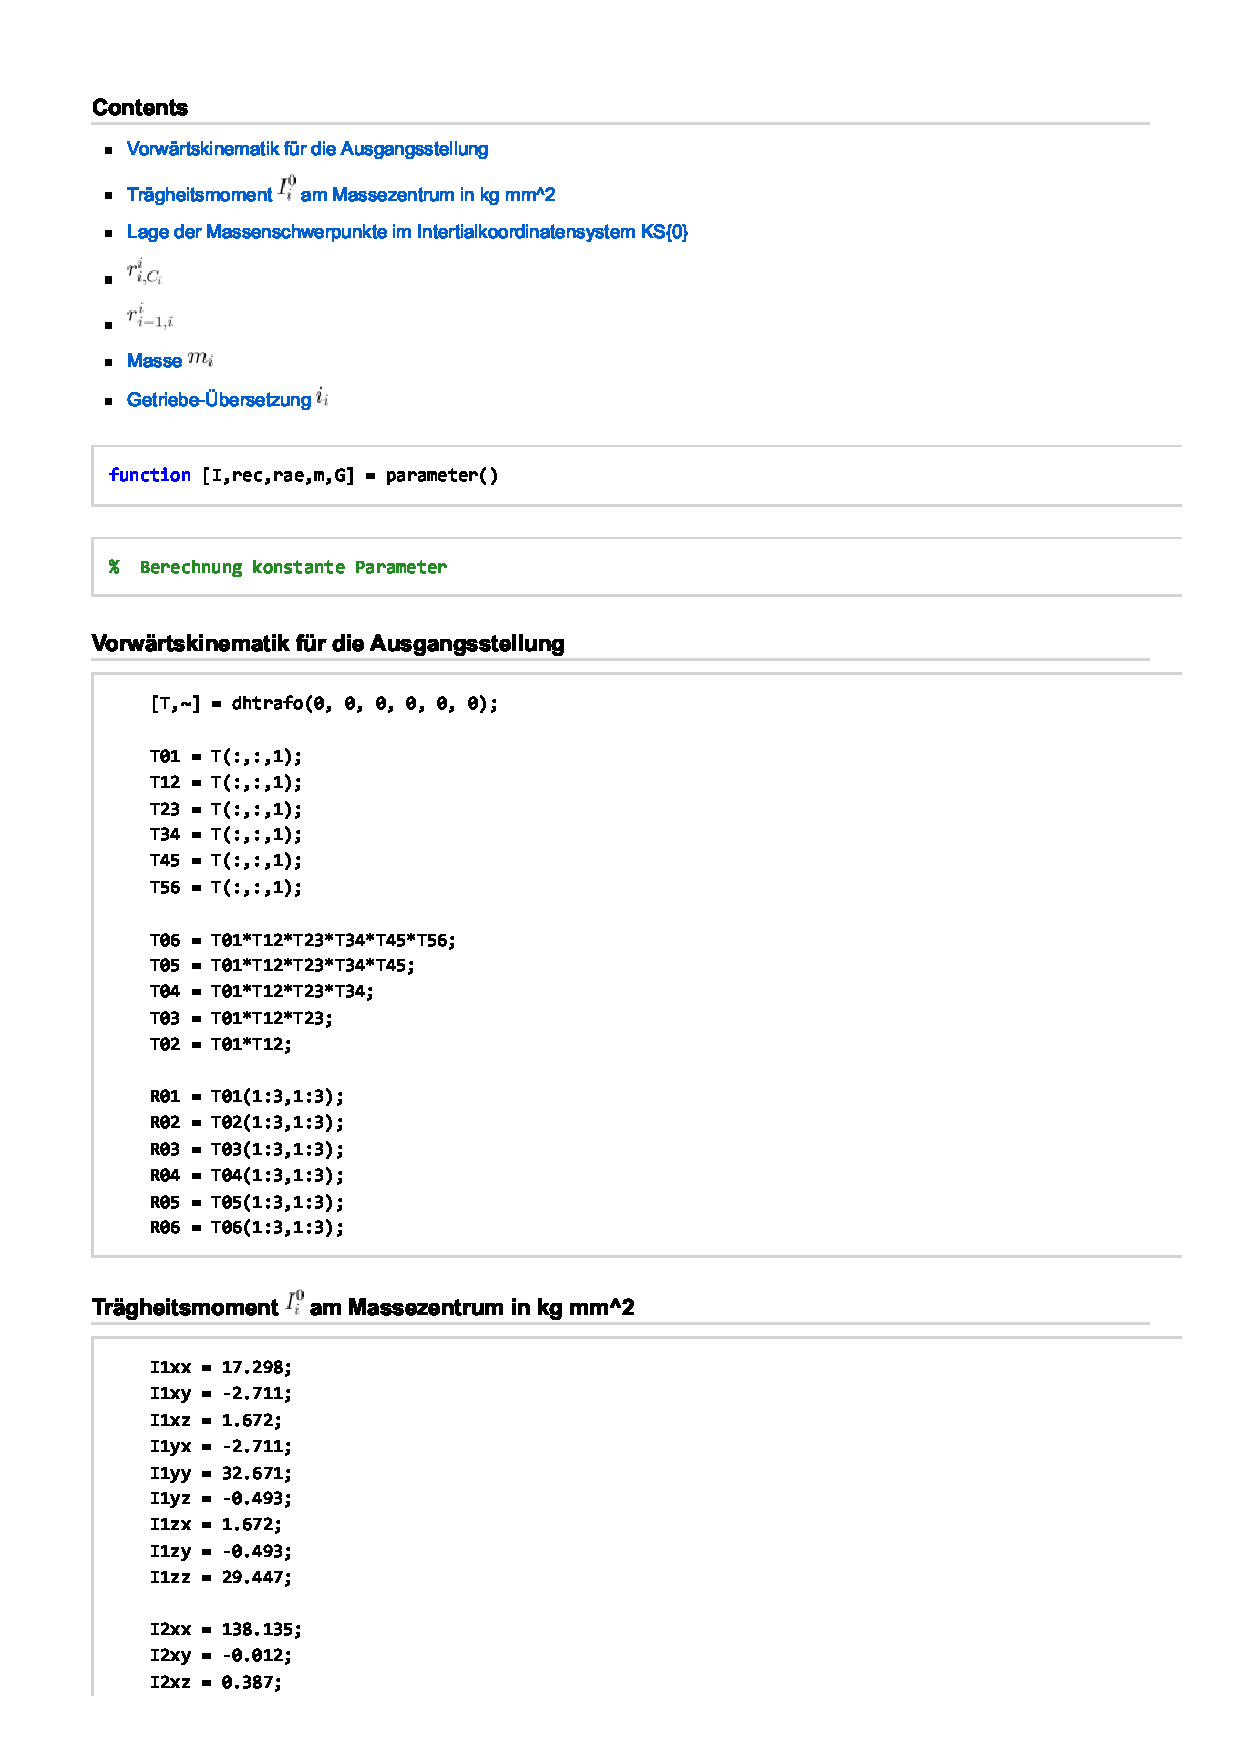
\includepdf[pages=1-4]{C:/Users/denni/Documents/Bachelorarbeit/BachelorThesis/literature/Anhang/parameter_matlab.pdf}
\setcounter{section}{1}
\section{Parameter}
\begin{lstlisting}[language=Matlab, numbers=none]
function [I,rec,rae,m,G] = parameter()
% Berechnung konstante Parameter
\end{lstlisting}
%
\subsection{Vorwärtskinematik für die Ausgangsstellung}
%
\begin{lstlisting}[language=Matlab, numbers=none]
[T,~,~] = dhtrafo(0, 0, 0, 0, 0, 0);

T01 = T(:,:,1);
T12 = T(:,:,2);
T23 = T(:,:,3);
T34 = T(:,:,4);
T45 = T(:,:,5);
T56 = T(:,:,6);
T06 = T01*T12*T23*T34*T45*T56;
T05 = T01*T12*T23*T34*T45;
T04 = T01*T12*T23*T34;
T03 = T01*T12*T23;
T02 = T01*T12;

R01 = T01(1:3,1:3);
R02 = T02(1:3,1:3);
R03 = T03(1:3,1:3);
R04 = T04(1:3,1:3);
R05 = T05(1:3,1:3);
R06 = T06(1:3,1:3);
\end{lstlisting}
%
\subsection{Trägheitsmoment $I^{0}_i$ am Massezentrum in $\dfrac{\mathrm{kg}}{m^2}$}
%
\begin{lstlisting}[language=Matlab, numbers=none]
I1xx = 17.298;
I1xy = -2.711;
I1xz = 1.672;
I1yx = -2.711;
I1yy = 32.671;
I1yz = -0.493;
I1zx = 1.672;
I1zy = -0.493;
I1zz = 29.447;

I2xx = 138.135;
I2xy = -0.012;
I2xz = 0.387;
I2yx = -0.012;
I2yy = 136.664;
I2yz = 9.231;
I2zx = 0.387;
I2zy = 9.231;
I2zz = 11.838;

I3xx = 3.031;
I3xy = -1.386;
I3xz = -0.045;
I3yx = -1.386;
I3yy = 30.03;
I3yz = -0.21;
I3zx = -0.045;
I3zy = -0.21;
I3zz = 29.693;

I4xx = 0.099;
I4xy = -0.032;
I4xz = -0.001;
I4yx = -0.032;
I4yy = 0.701;
I4yz = -9.367E-06;
I4zx = -0.001;
I4zy = -9.367E-06;
I4zz = 0.698;

I5xx = 0.481;
I5xy = 0.118;
I5xz = 0.00;
I5yx = 0.118;
I5yy = 0.424;
I5yz = 0.00;
I5zx = 0.00;
I5zy = 0.00;
I5zz = 0.675;

I6xx = 0.011;
I6xy = 5.143E-07;
I6xz = -2.003E-06;
I6yx = 5.143E-07;
I6yy = 0.006;
I6yz = 1.220E-07;
I6zx = -2.003E-06;
I6zy = 1.220E-07;
I6zz = 0.006;

% Ähnlichkeitstransformation zur Umrechung in die Körperfesten
% Koordinatensysteme

I1base = [ I1xx, I1xy, I1xz;
I1yx, I1yy, I1yz;
I1zx, I1zy, I1zz];

I1 = R01'*I1base*R01;

I2base = [ I2xx, I2xy, I2xz;
I2yx, I2yy, I2yz;
I2zx, I2zy, I2zz];

I2 = R02'*I2base*R02;

I3base = [ I3xx, I3xy, I3xz;
I3yx, I3yy, I3yz;
I3zx, I3zy, I3zz];

I3 = R03'*I3base*R03;

I4base = [ I4xx, I4xy, I4xz;
I4yx, I4yy, I4yz;
I4zx, I4zy, I4zz];

I4 = R04'*I4base*R04;

I5base = [ I5xx, I5xy, I5xz;
I5yx, I5yy, I5yz;
I5zx, I5zy, I5zz];

I5 = R05'*I5base*R05;

I6base = [ I6xx, I6xy, I6xz;
I6yx, I6yy, I6yz;
I6zx, I6zy, I6zz];

I6 = R06'*I6base*R06;

I = cat(3,I1,I2,I3,I4,I5,I6);
\end{lstlisting}
%
\subsection{Lage der Massenschwerpunkte im Intertialkoordinatensystem KS\{0\}}
%
\begin{lstlisting}[language=Matlab, numbers=none]
com1 = [-30.103; 4.41; 452.213]/1000;
com2 = [330.979; -222.585; 1094.239]/1000;
com3 = [705.894; -8.126; 1908.436]/1000;
com4 = [1383.185; 4.492; 1909.983]/1000;
com5 = [1601.767; 33.833; 1909.955]/1000;
com6 = [1743.222; -0.007; 1910.051]/1000;
\end{lstlisting}
%
\subsection{$r^{i}_{i,C_i}$}
%
\begin{lstlisting}[language=Matlab, numbers=none]
r1e_c1 = (T01)\[com1;1]; r1e_c1 = r1e_c1(1:3,1);
r2e_c2 = (T02)\[com2;1]; r2e_c2 = r2e_c2(1:3,1);
r3e_c3 = (T03)\[com3;1]; r3e_c3 = r3e_c3(1:3,1);
r4e_c4 = (T04)\[com4;1]; r4e_c4 = r4e_c4(1:3,1);
r5e_c5 = (T05)\[com5;1]; r5e_c5 = r5e_c5(1:3,1);
r6e_c6 = (T06)\[com6;1]; r6e_c6 = r6e_c6(1:3,1);
rec= cat(3, r1e_c1, r2e_c2, r3e_c3, r4e_c4, r5e_c5, r6e_c6);
\end{lstlisting}
%
\subsection{$r^{i}_{i-1,i}$}
%
\begin{lstlisting}[language=Matlab, numbers=none]
r1a_e = -inv(T01); r1a_e = r1a_e(1:3,4);
r2a_e = -inv(T12); r2a_e = r2a_e(1:3,4);
r3a_e = -inv(T23); r3a_e = r3a_e(1:3,4);
r4a_e = -inv(T34); r4a_e = r4a_e(1:3,4);
r5a_e = -inv(T45); r5a_e = r5a_e(1:3,4);
r6a_e = -inv(T56); r6a_e = r6a_e(1:3,4);
rae = cat(3, r1a_e, r2a_e, r3a_e, r4a_e, r5a_e, r6a_e);
\end{lstlisting}
%
\subsection{Masse $m_i$}
%
\begin{lstlisting}[language=Matlab, numbers=none]
m1 = 535;
m2 = 696.3;
m3 = 361.6; % +65.3 kg für die Schlauchpaket-Halterung +50 kg für die Antriebe 4 und 5;
m4 = 39.676;
m5 = 53.619;
m6 = 4.528;
m = [m1,m2,m3,m4,m5,m6];
\end{lstlisting}
%
\subsection{Getriebe-Übersetzung $i_i$}
%
\begin{lstlisting}[language=Matlab, numbers=none]
i1 = -7/1798;
i2 = -17/4576;
i3 = 3/754;
i4 = -55/10387;
i5 = -483/91834;
i6 = 49400/6485103;
G = [i1, i2, i3, i4, i5, i6];
\end{lstlisting}
%
\setcounter{section}{2}
\section{RNEA}
\label{add:rnea}
%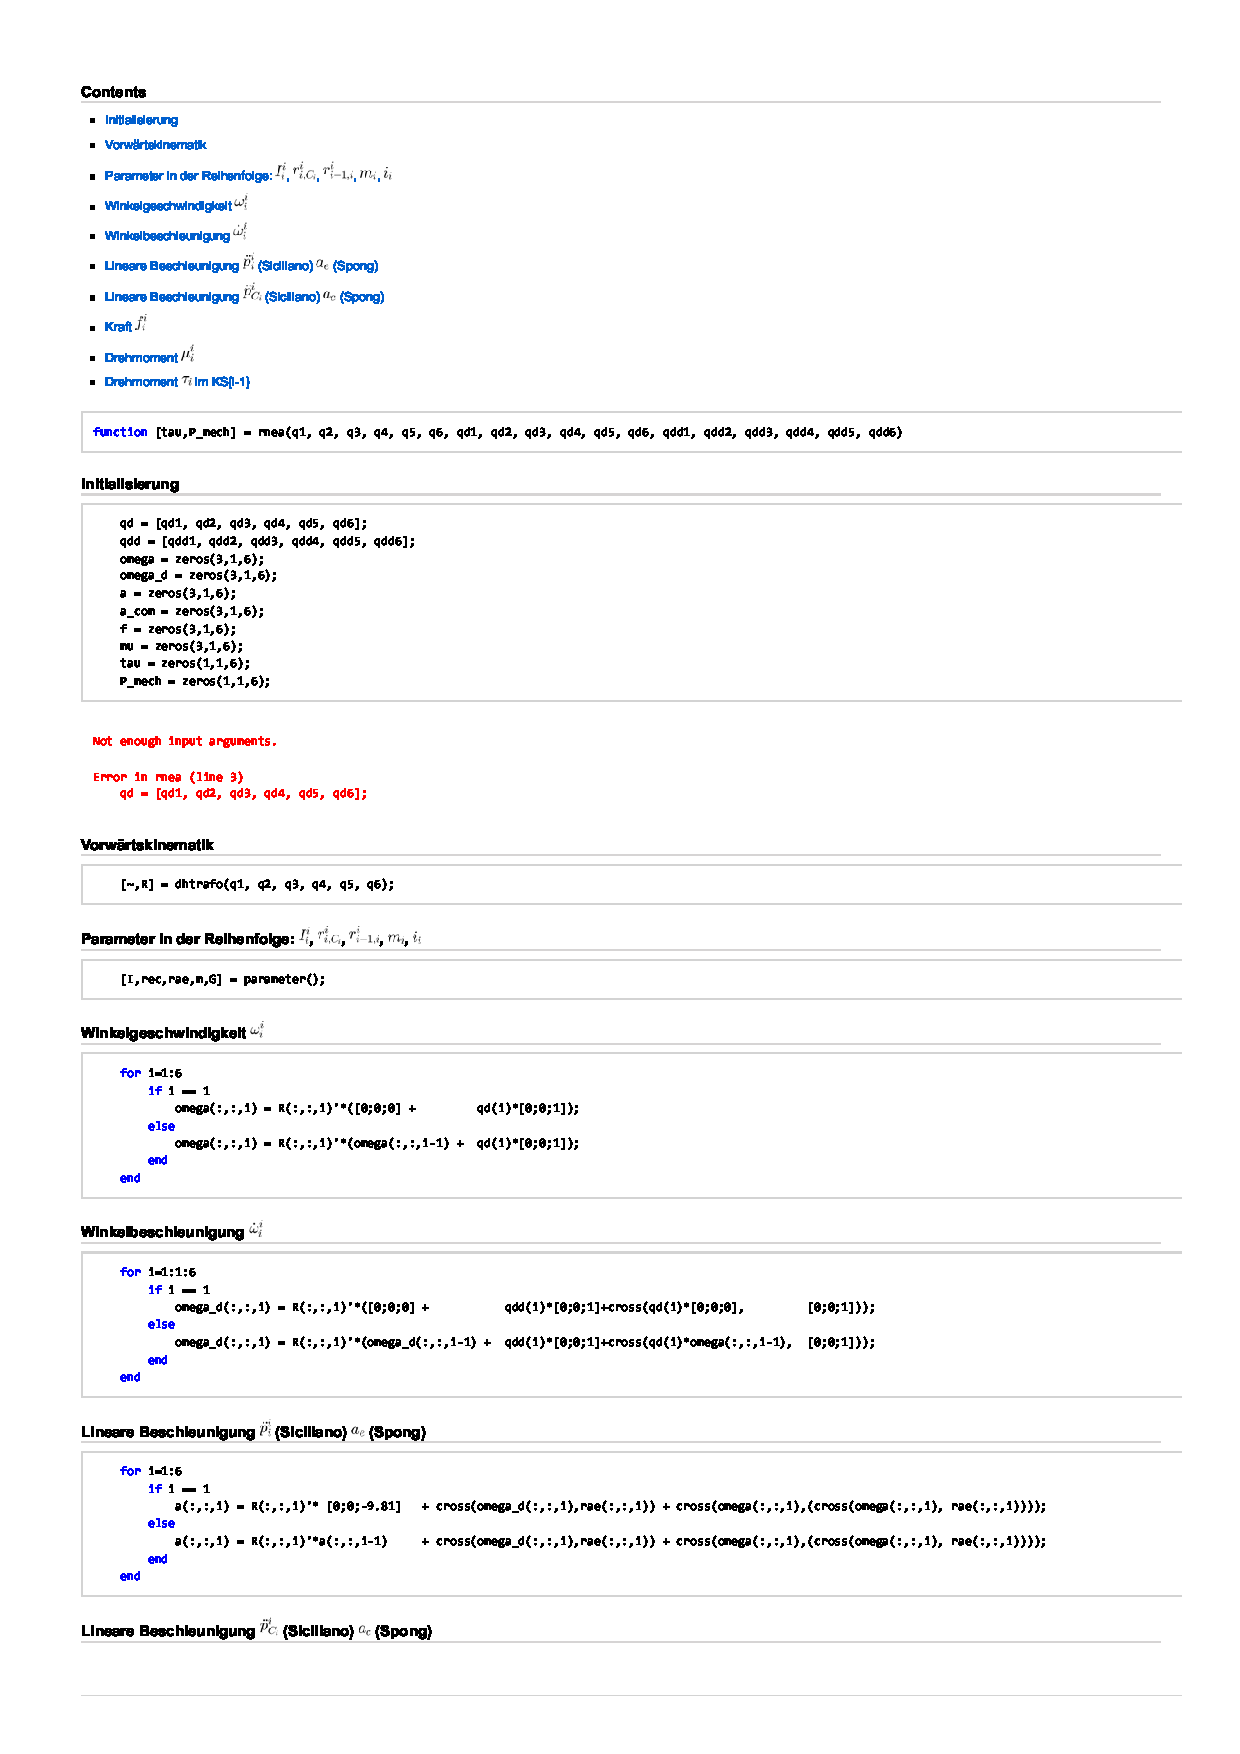
\includepdf[pages=1-2]{C:/Users/denni/Documents/Bachelorarbeit/BachelorThesis/literature/Anhang/rnea_matlab.pdf}
\begin{lstlisting}[language=Matlab, numbers=none]
function [tau,P_mech] = rnea(q1, q2, q3, q4, q5, q6, qd1, qd2, qd3, qd4, qd5, qd6, qdd1, qdd2, qdd3, qdd4, qdd5, qdd6)
\end{lstlisting}
%
\subsection{Initialisierung}
%
\begin{lstlisting}[language=Matlab, numbers=none]
qd = [qd1, qd2, qd3, qd4, qd5, qd6];
qdd = [qdd1, qdd2, qdd3, qdd4, qdd5, qdd6];
omega = zeros(3,1,6);
omega_d = zeros(3,1,6);
a = zeros(3,1,6);
a_com = zeros(3,1,6);
f = zeros(3,1,6);
mu = zeros(3,1,6);
tau = zeros(1,1,6);
P_mech = zeros(1,1,6);
\end{lstlisting}
%
\subsection{Vorwärtskinematik}
%
\begin{lstlisting}[language=Matlab, numbers=none]
[~,R,R0i] = dhtrafo(q1, q2, q3, q4, q5, q6);
\end{lstlisting}
%
\subsection{Parameter in der Reihenfolge: $I^{i}_{i}$, $r^{i}_{i,C_i}$, $r^{i}_{i-1,i}$, $m_i$, $i_i$}
%
\begin{lstlisting}[language=Matlab, numbers=none]
[I,rec,rae,m,G] = parameter();
\end{lstlisting}
%
\subsection{Winkelgeschwindigkeit $\omega^{i}_i$}
%
\begin{lstlisting}[language=Matlab, numbers=none]
for i=1:6
	if i == 1
		omega(:,:,i) = R(:,:,i)'*([0;0;0] + qd(i)*[0;0;1]);
	else
		omega(:,:,i) = R(:,:,i)'*(omega(:,:,i-1) + qd(i)*[0;0;1]);
	end
end
\end{lstlisting}
%
\subsection{Winkelbeschleunigung $\dot\omega^{i}_i$}
%
\begin{lstlisting}[language=Matlab, numbers=none]
for i=1:1:6
	if i == 1
		omega_d(:,:,i) = R(:,:,i)'*([0;0;0] + qdd(i)*[0;0;1]+cross(qd(i)*[0;0;0], [0;0;1]));
	else
		omega_d(:,:,i) = R(:,:,i)'*(omega_d(:,:,i-1) + qdd(i)*[0;0;1]+cross(qd(i)*omega(:,:,i-1), [0;0;1]));
	end
end
\end{lstlisting}
%
\subsection{Lineare Beschleunigung $\ddot p^{i}_i$ (Siciliano) $a_e$ (Spong)}
%
\begin{lstlisting}[language=Matlab, numbers=none]
for i=1:6
	if i == 1
		a(:,:,i) = R(:,:,i)'* [0;0;-9.81] + cross(omega_d(:,:,i),rae(:,:,i)) + cross(omega(:,:,i),(cross(omega(:,:,i), rae(:,:,i))));
	else
		a(:,:,i) = R(:,:,i)'*a(:,:,i-1) + cross(omega_d(:,:,i),rae(:,:,i)) + cross(omega(:,:,i),(cross(omega(:,:,i), rae(:,:,i))));
	end
end
\end{lstlisting}
%
\subsection{Lineare Beschleunigung $\ddot p^{i}_{C_i}$ (Siciliano) $a_c$ (Spong)}
%
\begin{lstlisting}[language=Matlab, numbers=none]
for i=1:1:6
	a_com(:,:,i) = a(:,:,i) + cross(omega_d(:,:,i),rec(:,:,i)) + cross(omega(:,:,i),(cross(omega(:,:,i), rec(:,:,i))));
end
\end{lstlisting}
%
\subsection{Gewichtsausgleich}
%
\begin{lstlisting}[language=Matlab, numbers=none]
F_gravity = zeros(3, 1, 6); % Vektor für die Gewichtskraft
	for i = 1:6
	F_gravity(:,:,i) = m(i) * [0; 0; -9.81]; % Gewichtskraft in Weltkoordinaten
	F_gravity(:,:,i) = R0i(:,:,i)' * F_gravity(:,:,i); % Gewichtskraft ins Körpersystem transformieren
end

for i = 3:-1:2
	if i == 3
		fgrav(:,:,i) = eye(3)*F_gravity(:,:,i);
		mugrav(:,:,i) = cross(-fgrav(:,:,i),(rae(:,:,i)+rec(:,:,i)));
	else
		fgrav(:,:,i) = R(:,:,i+1)*fgrav(:,:,i+1) + eye(3)*F_gravity(:,:,i);
		mugrav(:,:,i) = cross(-fgrav(:,:,i),(rae(:,:,i)+rec(:,:,i))) + R(:,:,i+1)*mugrav(:,:,i+1) + R(:,:,i+1)*cross(fgrav(:,:,i+1), rec(:,:,i));
	end
end
\end{lstlisting}
%
\subsection{Kraft $f^{i}_i$}
%
\begin{lstlisting}[language=Matlab, numbers=none]
for i = 6:-1:1
	if i == 6
		f(:,:,i) = eye(3)*[0;0;0] + m(i)*a_com(:,:,i);
	elseif i == 2
		f(:,:,i) = R(:,:,i+1)*f(:,:,i+1) + m(i)*a_com(:,:,i);
	else
		f(:,:,i) = R(:,:,i+1)*f(:,:,i+1) + m(i)*a_com(:,:,i);
	end
end
\end{lstlisting}
%
\subsection{Drehmoment $\mu^{i}_i$}
Übertragung des Drehmoments von der zweiten auf die ersten Achse ist zu Null gesetzt
\begin{lstlisting}[language=Matlab, numbers=none]
for i = 6:-1:1
	if i == 6
		mu(:,:,i) = cross(-f(:,:,i),(rae(:,:,i)+rec(:,:,i))) + eye(3)*[0;0;0] + eye(3)*cross([0;0;0], rec(:,:,i)) + I(:,:,i)*omega_d(:,:,i) + cross(omega(:,:,i),(I(:,:,i)*omega(:,:,i)));
	elseif i == 2
		mu(:,:,i) = cross(-f(:,:,i),(rae(:,:,i)+rec(:,:,i))) + R(:,:,i+1)*mu(:,:,i+1) + R(:,:,i+1)*cross(f(:,:,i+1), rec(:,:,i)) + I(:,:,i)*omega_d(:,:,i) + 	cross(omega(:,:,i),(I(:,:,i)*omega(:,:,i)))- mugrav(:,:,i);
	elseif i == 1
		mu(:,:,i) = cross(-f(:,:,i),(rae(:,:,i)+rec(:,:,i))) + R(:,:,i+1)*cross(f(:,:,i+1), rec(:,:,i)) + I(:,:,i)*omega_d(:,:,i) + 	cross(omega(:,:,i),(I(:,:,i)*omega(:,:,i)));
	else
		mu(:,:,i) = cross(-f(:,:,i),(rae(:,:,i)+rec(:,:,i))) + R(:,:,i+1)*mu(:,:,i+1) + R(:,:,i+1)*cross(f(:,:,i+1), rec(:,:,i)) + I(:,:,i)*omega_d(:,:,i) + 	cross(omega(:,:,i),(I(:,:,i)*omega(:,:,i)));
	end
end
\end{lstlisting}
%
\subsection{Drehmoment $\tau_i$ im KS\{i-1\}}
%
\begin{lstlisting}[language=Matlab, numbers=none]
for i = 1:1:6
	tau(i) = transpose(mu(:,:,i)) * transpose(R(:,:,i))*[0;0;1];%* G(i)
end

for i = 1:1:6
	P_mech(i) = tau(i)*qd(i);%/G(i);
end
end
\end{lstlisting}
\setcounter{section}{3}
\section{Bahnplanung}
\label{add:traj}
%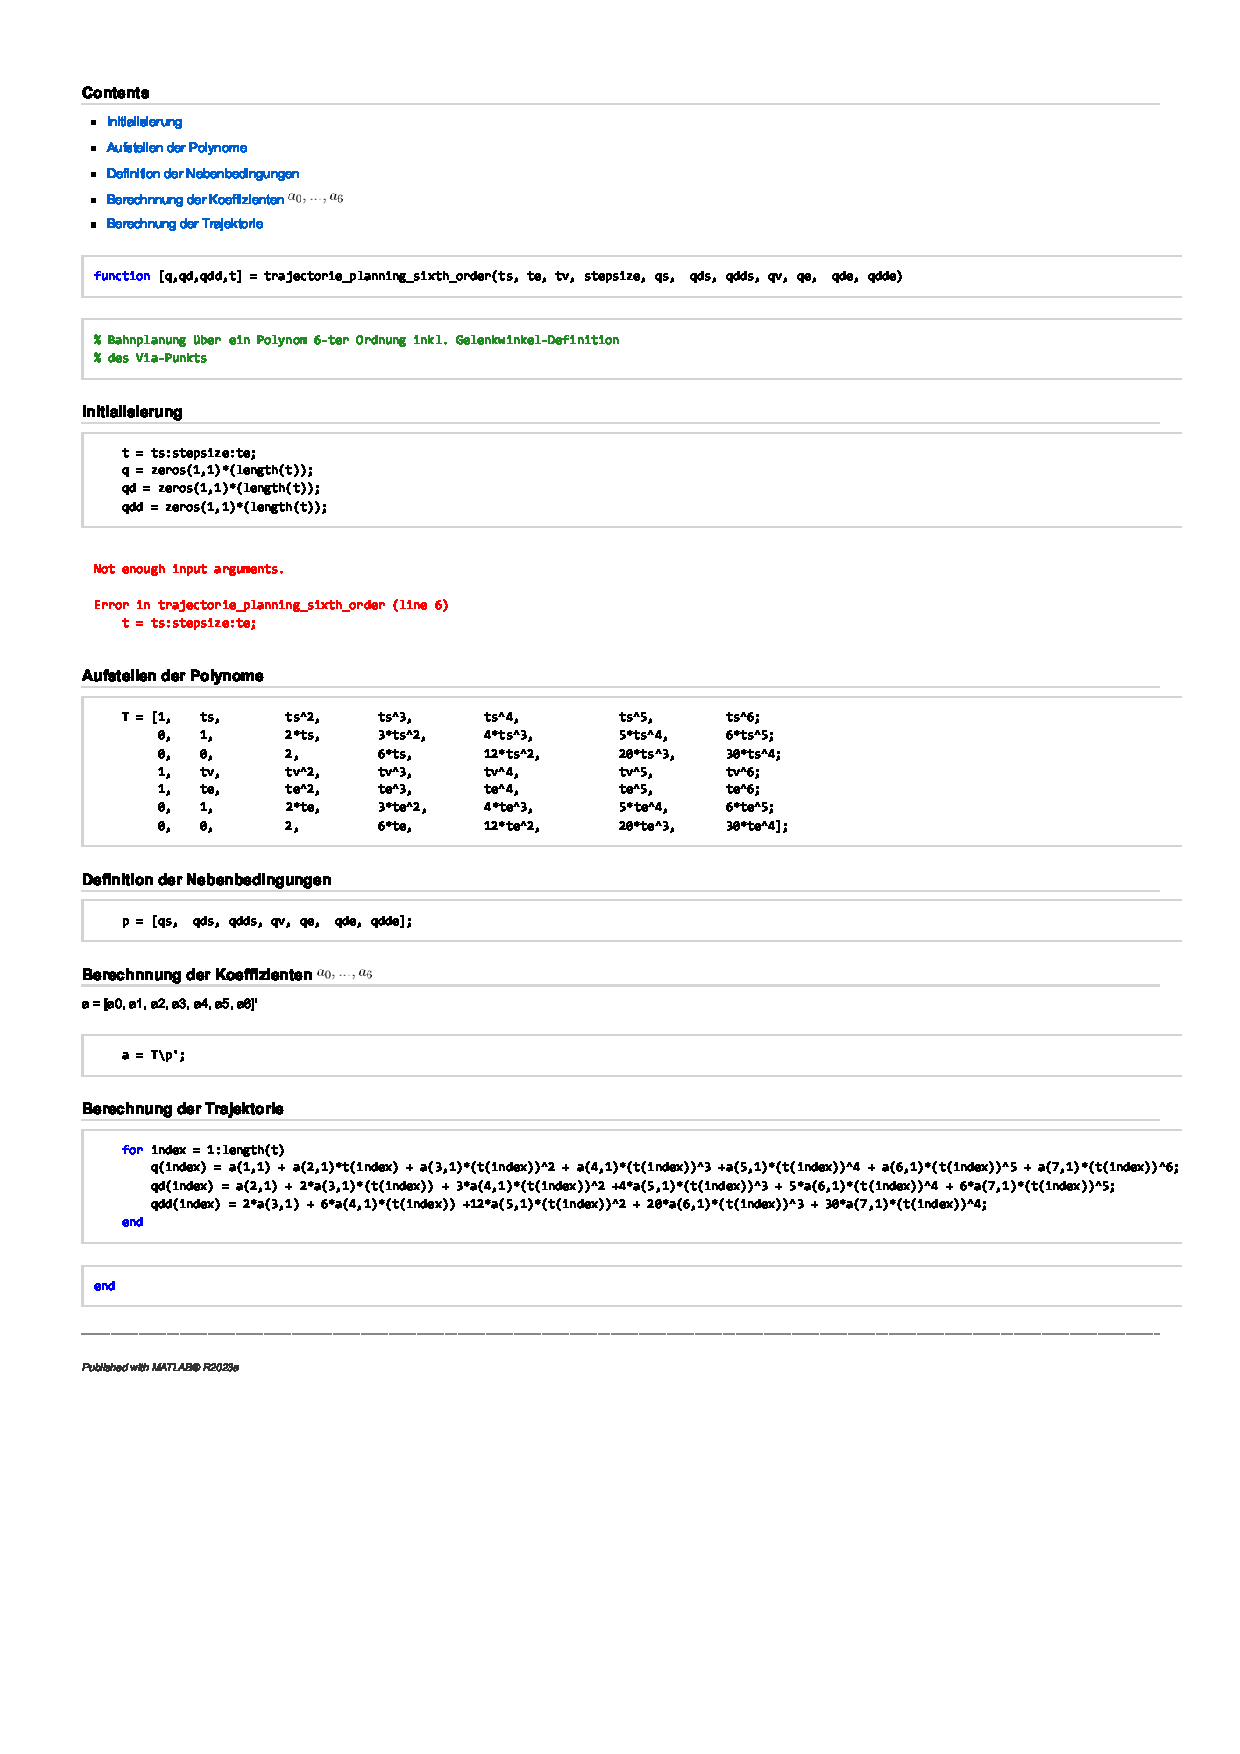
\includepdf[pages=1]{C:/Users/denni/Documents/Bachelorarbeit/BachelorThesis/literature/Anhang/trajectorie_planning_sixth_order_matlab.pdf}
\begin{lstlisting}[language=Matlab, numbers=none]
function [q,qd,qdd,t] = trajectorie_planning_sixth_order(ts, te, tv, stepsize, qs, qds, qdds, qv, qe, qde, qdde)
% Bahnplanung über ein Polynom 6-ter Ordnung inkl. Gelenkwinkel-Definition des Via-P\dfrac
\end{lstlisting}
%
\subsection{Initialisierung}
%
\begin{lstlisting}[language=Matlab, numbers=none]
t = ts:stepsize:te;
q = zeros(1,1)*(length(t));
qd = zeros(1,1)*(length(t));
qdd = zeros(1,1)*(length(t));
\end{lstlisting}
%
\subsection{Aufstellen der Polynome}
%
\begin{lstlisting}[language=Matlab, numbers=none]
T =    [1, ts, 	ts^2, 	ts^3, 	ts^4, 		ts^5, 		ts^6;
				0, 1, 	2*ts, 	3*ts^2, 4*ts^3, 	5*ts^4, 	6*ts^5;
				0, 0, 	2, 		6*ts, 	12*ts^2,	20*ts^3,	30*ts^4;
				1, tv, 	tv^2, 	tv^3, 	tv^4, 		tv^5, 		tv^6;
				1, te, 	te^2, 	te^3, 	te^4, 		te^5, 		te^6;
				0, 1, 	2*te, 	3*te^2, 4*te^3, 	5*te^4,	 	6*te^5;
				0, 0, 	2, 		6*te, 	12*te^2,	20*te^3,	30*te^4];
\end{lstlisting}
%
\subsection{Definition der Nebenbedingungen}
%
\begin{lstlisting}[language=Matlab, numbers=none]
p = [qs, qds, qdds, qv, qe, qde, qdde];
\end{lstlisting}
%
\subsection{Berechnnung der Koeffizienten $a_0,...,a_6$}
%
\begin{par}
	a = [a0, a1, a2, a3, a4, a5, a6]'
\end{par} \vspace{1em}
\begin{lstlisting}[language=Matlab, numbers=none]
a = T\p';
\end{lstlisting}
%
\subsection{Berechnung der Trajektorie}
%
\begin{lstlisting}[language=Matlab, numbers=none]
for index = 1:length(t)
q(index) = a(1,1) + a(2,1)*t(index) + a(3,1)*(t(index))^2 + a(4,1)*(t(index))^3 +a(5,1)*(t(index))^4 + a(6,1)*(t(index))^5 + a(7,1)*(t(index))^6;
qd(index) = a(2,1) + 2*a(3,1)*(t(index)) + 3*a(4,1)*(t(index))^2 +4*a(5,1)*(t(index))^3 + 5*a(6,1)*(t(index))^4 + 6*a(7,1)*(t(index))^5;
qdd(index) = 2*a(3,1) + 6*a(4,1)*(t(index)) +12*a(5,1)*(t(index))^2 + 20*a(6,1)*(t(index))^3 + 30*a(7,1)*(t(index))^4;
end
\end{lstlisting}
%
\setcounter{section}{4}
\section{Testsimulation Bahnplanung}
\label{add:sim}
%
\subsection{Trajektorie Kleben-Seitenwand}
%
\begin{lstlisting}[language=Matlab, numbers=none]
te = 1.2; % Bewegungsdauer
\end{lstlisting}
%
\subsection{Bewegung 1 (home -\ensuremath{>} Vorposition)}
%
\begin{par}
	\% Startwert Gelenkwinkel qs1 = deg2rad(-7.61); qs2 = deg2rad(-119.27); qs3 = deg2rad(88.49-90); qs4 = deg2rad(10.27); qs5 = deg2rad(32.41); qs6 = deg2rad(-10.19);
\end{par} \vspace{1em}
\begin{par}
	\% Zielwert Gelenkwinkel qe1 = deg2rad(-14.83); qe2 = deg2rad(-105.81); qe3 = deg2rad(136.16-90); qe4 = deg2rad(-27.67); qe5 = deg2rad(-33.44); qe6 = deg2rad(22.89);
\end{par} \vspace{1em}
\begin{lstlisting}[language=Matlab, numbers=none]
% optimierte Via-Punkte
% qvd = [];
% qv1 = deg2rad(qvd(1));
% qv2 = deg2rad(qvd(2));
% qv3 = deg2rad(qvd(3));
% qv4 = deg2rad(qvd(4));
% qv5 = (deg2rad(qvd(5))+(qs5+qe5)*1/2)*1/2; % Für den Fall, dass der Wert zu dicht an den Grenzen liegt, was eine hohe Beschleunigung zur Folge hat, wird das Mittel aus dem optimierten und dem initialen Via-Punkt gebildet
% qv6 = (deg2rad(qvd(6))+(qs6+qe6)*1/2)*1/2;
\end{lstlisting}
%
\subsection{Bewegung 3 (letzter Punkt der Trajektorie Kleben Seitenwand -\ensuremath{>} home)}
%
\begin{par}
	Startwert Gelenkwinkel
\end{par} \vspace{1em}
\begin{lstlisting}[language=Matlab, numbers=none]
qs1 = deg2rad(-53.8);
qs2 = deg2rad(-70.34);
qs3 = deg2rad(98.82-90);
qs4 = deg2rad(-69.87);
qs5 = deg2rad(-58.7);
qs6 = deg2rad(55.7);

% Zielwert Gelenkwinkel
qe1 = deg2rad(-7.61);
qe2 = deg2rad(-119.27);
qe3 = deg2rad(88.49-90);
qe4 = deg2rad(10.27);
qe5 = deg2rad(32.41);
qe6 = deg2rad(-10.19);

% % Startwert Via-Punkte
% qv1 = (qs1+qe1)*1/2;
% qv2 = (qs2+qe2)*1/2;
% qv3 = (qs3+qe3)*1/2;
% qv4 = (qs4+qe4)*1/2;
% qv5 = (qs5+qe5)*1/2;
% qv6 = (qs6+qe6)*1/2;

% optimierte Via-Punkte
qvu = [-25.0007 -96.0711 8.8200 10.2700 -47.7822 -10.1900];
qv1 = deg2rad(qvu(1));
qv2 = deg2rad(qvu(2));
qv3 = deg2rad(qvu(3));
qv4 = (deg2rad(qvu(4))+(qs4+qe4)*1/2)*1/2;
qv5 = (deg2rad(qvu(5))+(qs5+qe5)*1/2)*1/2;
qv6 = (deg2rad(qvu(6))+(qs6+qe6)*1/2)*1/2;
\end{lstlisting}
%
\subsection{Bahnplanung}
%
\begin{lstlisting}[language=Matlab, numbers=none]
stepsize = 0.004;
ts = 0; % Startzeit
tv = (te-ts)/2; % Via-Punkt Zeitpunkt

% Start- und Endgeschwindigkeiten
qds1 = 0; qde1 = 0;
qds2 = 0; qde2 = 0;
qds3 = 0; qde3 = 0;
qds4 = 0; qde4 = 0;
qds5 = 0; qde5 = 0;
qds6 = 0; qde6 = 0;

% Start- und Endbeschleunigungen
qdds1 = 0; qdde1 = 0;
qdds2 = 0; qdde2 = 0;
qdds3 = 0; qdde3 = 0;
qdds4 = 0; qdde4 = 0;
qdds5 = 0; qdde5 = 0;
qdds6 = 0; qdde6 = 0;

qs = [qs1,qs2,qs3,qs4,qs5,qs6];
qe = [qe1,qe2,qe3,qe4,qe5,qe6];
qv = [qv1,qv2,qv3,qv4,qv5,qv6];
qds = [qds1,qds2,qds3,qds4,qds5,qds6];
qdds = [qdds1,qdds2,qdds3,qdds4,qdds5,qdds6];
qde = [qde1,qde2,qde3,qde4,qde5,qde6];
qdde = [qdde1,qdde2,qdde3,qdde4,qdde5,qdde6];

% Bahnplanung Polynom 6-Ordnung
[q1,qd1,qdd1,~] = trajectorie_planning_sixth_order(ts, te, tv, stepsize, qs(1), qds(1), qdds(1), qv(1), qe(1), qde(1), qdde(1));
[q2,qd2,qdd2,~] = trajectorie_planning_sixth_order(ts, te, tv, stepsize, qs(2), qds(2), qdds(2), qv(2), qe(2), qde(2), qdde(2));
[q3,qd3,qdd3,~] = trajectorie_planning_sixth_order(ts, te, tv, stepsize, qs(3), qds(3), qdds(3), qv(3), qe(3), qde(3), qdde(3));
[q4,qd4,qdd4,~] = trajectorie_planning_sixth_order(ts, te, tv, stepsize, qs(4), qds(4), qdds(4), qv(4), qe(4), qde(4), qdde(4));
[q5,qd5,qdd5,~] = trajectorie_planning_sixth_order(ts, te, tv, stepsize, qs(5), qds(5), qdds(5), qv(5), qe(5), qde(5), qdde(5));
[q6,qd6,qdd6,t] = trajectorie_planning_sixth_order(ts, te, tv, stepsize, qs(6), qds(6), qdds(6), qv(6), qe(6), qde(6), qdde(6));
\end{lstlisting}
%
\subsection{Modellberechnung der Drehmomente, Leistungsaufnahme}
%
\begin{lstlisting}[language=Matlab, numbers=none]
% Initialisierung
tau = zeros(length(t));
Pmech = zeros(length(t));
Pmech_diss = zeros(length(t));
Pmech_sink = zeros(length(t));

% RNEA
for index = 1:1:(length(t))
[ret_tau,ret_Pmech] = rnea(q1(index), q2(index), q3(index), q4(index), q5(index), q6(index), qd1(index), qd2(index), qd3(index), qd4(index), qd5(index), qd6(index), qdd1(index), qdd2(index), qdd3(index), qdd4(index), qdd5(index), qdd6(index));
tau(index,1) = ret_tau(1);
tau(index,2) = ret_tau(2);
tau(index,3) = ret_tau(3);
tau(index,4) = ret_tau(4);
tau(index,5) = ret_tau(5);
tau(index,6) = ret_tau(6);
Pmech(index,1) = ret_Pmech(1);
Pmech(index,2) = ret_Pmech(2);
Pmech(index,3) = ret_Pmech(3);
Pmech(index,4) = ret_Pmech(4);
Pmech(index,5) = ret_Pmech(5);
Pmech(index,6) = ret_Pmech(6);
end
\end{lstlisting}
%
\subsection{Daten Vorverarbeitung}
%
\begin{lstlisting}[language=Matlab, numbers=none]
for index = 1:1:(length(t))
	for var = 1:6
		if Pmech(index,var) > 0
			Pmech_sink(index,var) = Pmech(index,var);
		else
			Pmech_diss(index,var) = Pmech(index,var);
			Pmech_sink(index,var) = 0;
		end
	end
end
\end{lstlisting}
%
\subsection{Anzeige der Daten}
%
\begin{lstlisting}[language=Matlab, numbers=none]
disp('qv1');disp(rad2deg(qv1));
disp('qv2');disp(rad2deg(qv2));
disp('qv3');disp(rad2deg(qv3));
disp('qv4');disp(rad2deg(qv4));
disp('qv5');disp(rad2deg(qv5));
disp('qv6');disp(rad2deg(qv6));
torque = sum(sum(abs(tau)))/length(t); disp('Mittelwert der Summe des Betrags der Getriebe-Drehmomente in Nm'); disp(torque);
P_mech = sum(sum((Pmech_sink))/length(t)); disp('Mittelwert der aufgenommenen mechanischen Leistung in W'); disp(P_mech);
P_mech_diss = sum(sum((Pmech_diss))/length(t))*(te-ts); disp('Dissipierte Energie in J'); disp(P_mech_diss);
E_mech = sum(sum(Pmech_sink)/length(t))*(te-ts); disp('Aufgenommene Energie in J'); disp(E_mech);
\end{lstlisting}
%
\subsection{Erzeuge die Abbildungen}
%
\begin{lstlisting}[language=Matlab, numbers=none]
show_graphics(q1, q2, q3, q4, q5, q6, qd1, qd2, qd3, qd4, qd5, qd6, qdd1, qdd2, qdd3, qdd4, qdd5, qdd6, t, tau, Pmech)
\end{lstlisting}
%
%
\setcounter{section}{5}
\section{Optimierung}
\label{add:optimierer}
%
\subsection{KlebenSeitenwand}
%
\subsection{Bewegung 1 (home -\ensuremath{>} Vorposition)}
%
\begin{par}
	\% Startwert Gelenkwinkel qs1 = deg2rad(-7.61); qs2 = deg2rad(-119.27); qs3 = deg2rad(88.49-90); qs4 = deg2rad(10.27); qs5 = deg2rad(32.41); qs6 = deg2rad(-10.19);
\end{par} \vspace{1em}
\begin{par}
	\% Zielwert Gelenkwinkel qe1 = deg2rad(-14.83); qe2 = deg2rad(-105.81); qe3 = deg2rad(136.16-90); qe4 = deg2rad(-27.67); qe5 = deg2rad(-33.44); qe6 = deg2rad(22.89);
\end{par} \vspace{1em}
%
\subsection{Bewegung 3 (letzter Punkt der Trajektorie Kleben Seitenwand -\ensuremath{>} home)}
%
\begin{par}
	Startwert Gelenkwinkel
\end{par} \vspace{1em}
\begin{lstlisting}[language=Matlab, numbers=none]
qs1 = deg2rad(-53.8);
qs2 = deg2rad(-70.34);
qs3 = deg2rad(98.82-90);
qs4 = deg2rad(-69.87);
qs5 = deg2rad(-58.7);
qs6 = deg2rad(55.7);

% Zielwert Gelenkwinkel
qe1 = deg2rad(-7.61);
qe2 = deg2rad(-119.27);
qe3 = deg2rad(88.49-90);
qe4 = deg2rad(10.27);
qe5 = deg2rad(32.41);
qe6 = deg2rad(-10.19);
\end{lstlisting}
%
\subsection{Startwert Via-Punkte}
%
\begin{lstlisting}[language=Matlab, numbers=none]
denum = 1; % Testen von Startwerten, die von Mittelpunkt abweichen
qv1 = (qs1+qe1)*1/2;%-(abs(qs1-qe1)/2)/denum;
qv2 = (qs2+qe2)*1/2;%-(abs(qs1-qe1)/2)/denum;
qv3 = (qs3+qe3)*1/2;%-(abs(qs1-qe1)/2)/denum;
qv4 = (qs4+qe4)*1/2;%-(abs(qs1-qe1)/2)/denum;
qv5 = (qs5+qe5)*1/2;%-(abs(qs1-qe1)/2)/denum;
qv6 = (qs6+qe6)*1/2;%-(abs(qs1-qe1)/2)/denum;
\end{lstlisting}
%
\subsection{Initial-Trajektorie-Definition}
%
\begin{lstlisting}[language=Matlab, numbers=none]
te = 1.2;
qs = [qs1,qs2,qs3,qs4,qs5,qs6];
qe = [qe1,qe2,qe3,qe4,qe5,qe6];
qv = [qv1,qv2,qv3,qv4,qv5,qv6];
\end{lstlisting}
%
\subsection{Definition Optimierer}
%
\begin{par}
	Zielfunktion
\end{par} \vspace{1em}
\begin{lstlisting}[language=Matlab, numbers=none]
objective = @(qv) calc_objective(qs,qe,qv,te);
% Startwert
x0 = qv;
% Anzeige des Energieverbrauchs beim Start der Optimierung
disp(['initial Objective: ' num2str(objective(x0))]);
% Gleichungsnebenbedingungen
A = [];
b = [];
% Ungleichungssnebenbedingungen
Aeq = [];
beq = [];
% Grenzen des Parametervektors
lb = (qv-(abs(qs-qe))/2);
ub = (qv+(abs(qs-qe))/2);
% Nichtlineare Nebenbedingungen
nonlcon = [];
% Auswahl des Solvers fmincon
% Algorithmus sequentielle quadratische Programmierung
% max. Anzahl der Iterationen = 25
% und Ausgabe des Zielfunktionswertes mit jeder Iteration
options = optimoptions(@fmincon,'Algorithm','sqp', 'MaxIterations', 25,'PlotFcn',@optimplotfval);
% Ausführen der Optimierung
[x,fval,ef,output,lambda] = fmincon(objective,x0,A,b,Aeq,beq,lb,ub,nonlcon,options);
% Anzeige des energieoptimierten Parametervektors
disp(x*180/pi)
\end{lstlisting}
\color{lightgray} \begin{lstlisting}[language=Matlab, numbers=none]
% Startwert
E in J
2.0013e+03

% Zielwert
E in J
1.8074e+03

% identifzierter Parametervektor
-24.8857 -96.0716 8.8200 10.2700 -47.5666 -10.1900
\end{lstlisting} \color{black}
%
%\section{MATLAB Optimization Toolbox Functions}
%\label{add:OptimizationToolbox}
%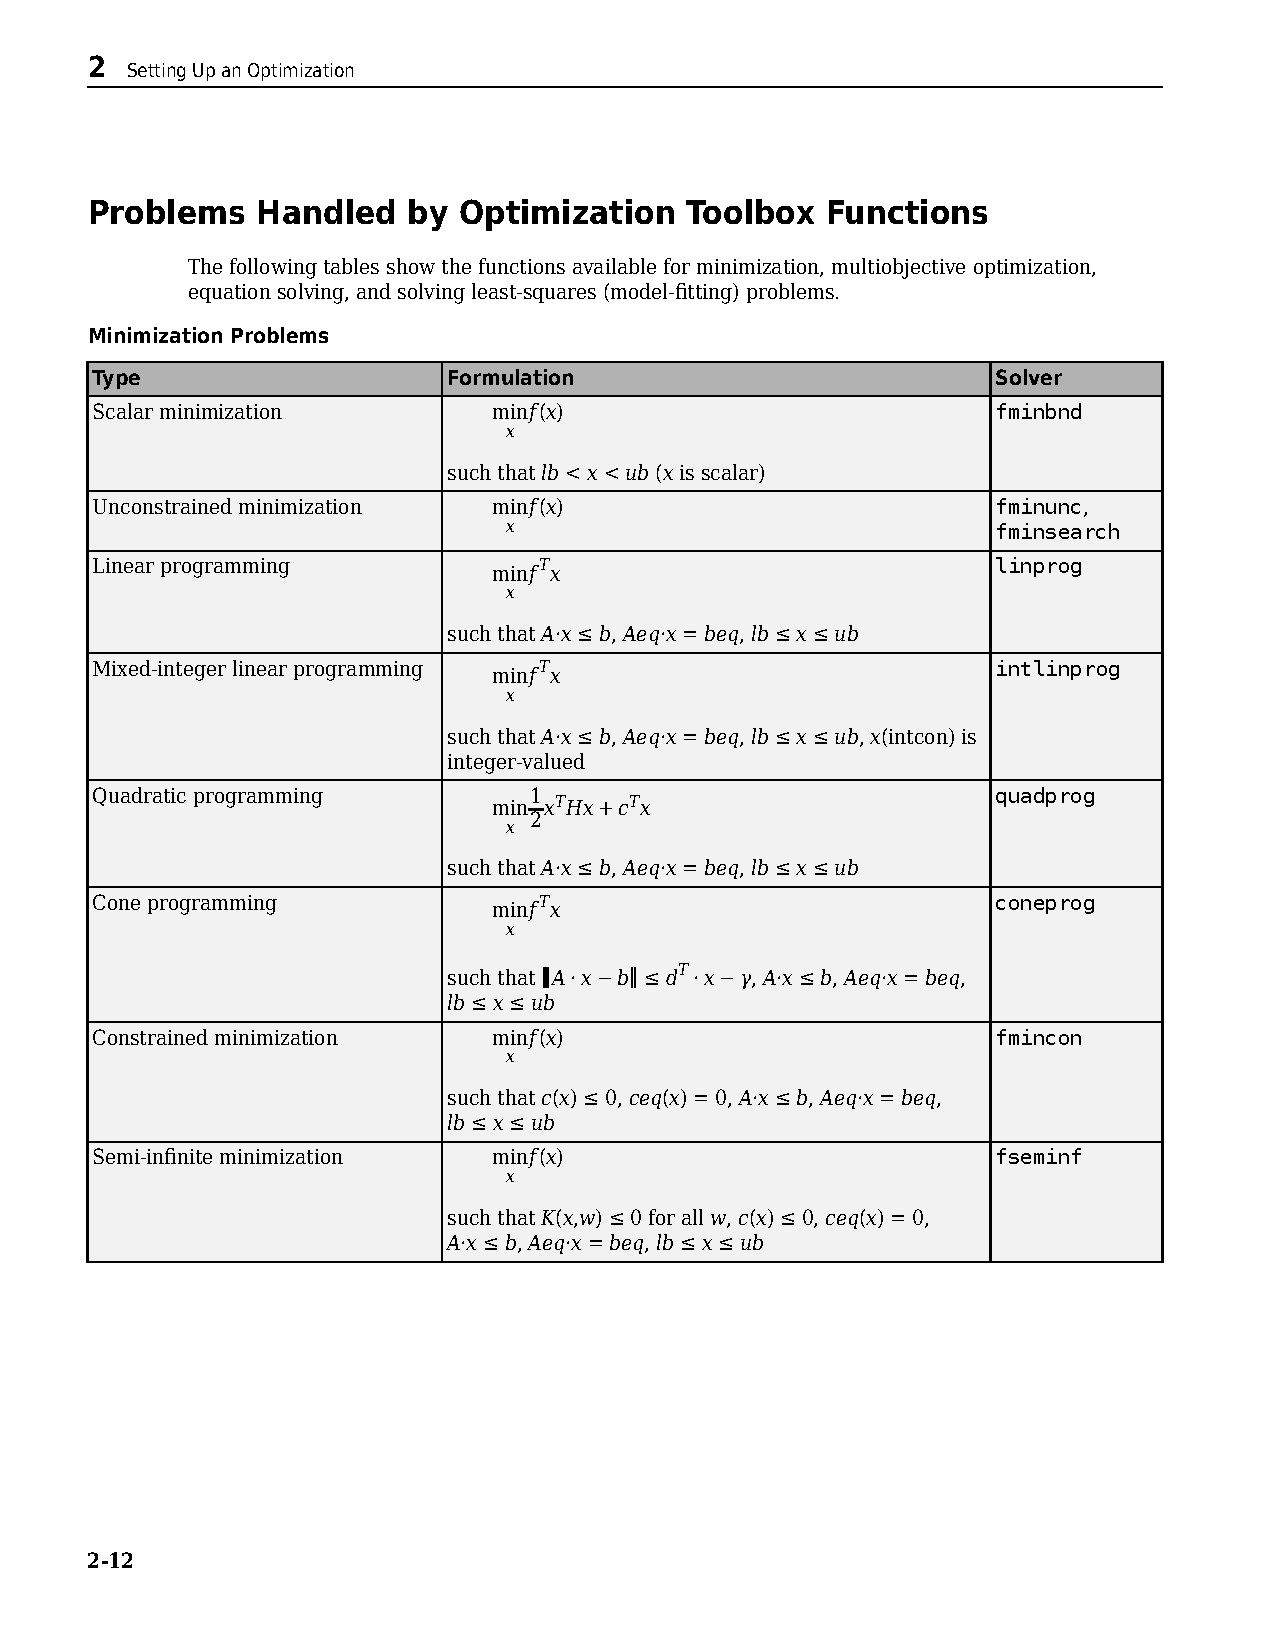
\includepdf[pages=1]{C:/Users/denni/Documents/Bachelorarbeit/BachelorThesis/literature/Anhang/OptimizationToolbox}
%
\setcounter{section}{6}
\section{Berechnung der Zielfunktion}
%
\label{add:zielfunktion}
\begin{lstlisting}[language=Matlab, numbers=none]
function [E_mech] = calc_objective(qs,qe,qv,te)
\end{lstlisting}
\begin{lstlisting}[language=Matlab, numbers=none]
% Berechung der Zielfunktion (Energieverbrauch) über die nicht
% dissipierte mechanische Leistung
\end{lstlisting}
%
\subsection{Bahnplanung}
%
\begin{lstlisting}[language=Matlab, numbers=none]
stepsize = 0.004;
ts = 0;
tv = (te-ts)/2;

qds1 = 0; qde1 = 0;
qds2 = 0; qde2 = 0;
qds3 = 0; qde3 = 0;
qds4 = 0; qde4 = 0;
qds5 = 0; qde5 = 0;
qds6 = 0; qde6 = 0;

qdds1 = 0; qdde1 = 0;
qdds2 = 0; qdde2 = 0;
qdds3 = 0; qdde3 = 0;
qdds4 = 0; qdde4 = 0;
qdds5 = 0; qdde5 = 0;
qdds6 = 0; qdde6 = 0;

qds = [qds1,qds2,qds3,qds4,qds5,qds6];
qdds = [qdds1,qdds2,qdds3,qdds4,qdds5,qdds6];
qde = [qde1,qde2,qde3,qde4,qde5,qde6];
qdde = [qdde1,qdde2,qdde3,qdde4,qdde5,qdde6];

[q1,qd1,qdd1,~] = trajectorie_planning_sixth_order(ts, te, tv, stepsize, qs(1), qds(1), qdds(1), qv(1), qe(1), qde(1), qdde(1));
[q2,qd2,qdd2,~] = trajectorie_planning_sixth_order(ts, te, tv, stepsize, qs(2), qds(2), qdds(2), qv(2), qe(2), qde(2), qdde(2));
[q3,qd3,qdd3,~] = trajectorie_planning_sixth_order(ts, te, tv, stepsize, qs(3), qds(3), qdds(3), qv(3), qe(3), qde(3), qdde(3));
[q4,qd4,qdd4,~] = trajectorie_planning_sixth_order(ts, te, tv, stepsize, qs(4), qds(4), qdds(4), qv(4), qe(4), qde(4), qdde(4));
[q5,qd5,qdd5,~] = trajectorie_planning_sixth_order(ts, te, tv, stepsize, qs(5), qds(5), qdds(5), qv(5), qe(5), qde(5), qdde(5));
[q6,qd6,qdd6,t] = trajectorie_planning_sixth_order(ts, te, tv, stepsize, qs(6), qds(6), qdds(6), qv(6), qe(6), qde(6), qdde(6));
\end{lstlisting}
%
\subsection{Modellberechnung der Drehmomente, Leistungsaufnahme}
%
\begin{lstlisting}[language=Matlab, numbers=none]
% Initialisierung
tau = zeros(length(t));
Pmech = zeros(length(t));
Pmech_diss = zeros(length(t));
Pmech_sink = zeros(length(t));

for index = 1:1:(length(t))
[ret_tau,ret_Pmech] = rnea(q1(index), q2(index), q3(index), q4(index), q5(index), q6(index), qd1(index), qd2(index), qd3(index), qd4(index), qd5(index), qd6(index), qdd1(index), qdd2(index), qdd3(index), qdd4(index), qdd5(index), qdd6(index));
tau(index,1) = ret_tau(1);
tau(index,2) = ret_tau(2);
tau(index,3) = ret_tau(3);
tau(index,4) = ret_tau(4);
tau(index,5) = ret_tau(5);
tau(index,6) = ret_tau(6);
Pmech(index,1) = ret_Pmech(1);
Pmech(index,2) = ret_Pmech(2);
Pmech(index,3) = ret_Pmech(3);
Pmech(index,4) = ret_Pmech(4);
Pmech(index,5) = ret_Pmech(5);
Pmech(index,6) = ret_Pmech(6);
end
\end{lstlisting}
%
\subsection{Daten Vorverarbeitung}
%
\begin{lstlisting}[language=Matlab, numbers=none]
for index = 1:1:(length(t))
for var = 1:6
if Pmech(index,var) > 0
Pmech_sink(index,var) = Pmech(index,var);
else
Pmech_diss(index,var) = Pmech(index,var);
Pmech_sink(index,var) = 0;
end
end
end
\end{lstlisting}
%
\subsection{Anzeige der Daten}
%
\begin{lstlisting}[language=Matlab, numbers=none]
torque = sum(sum((tau).^2))/length(t);
E_mech = sum(sum((Pmech_sink))/length(t))*(te-ts); disp('E in J'); disp(E_mech);
\end{lstlisting}
%
%
\addchap{Anhang D - Messdaten}
\setcounter{chapter}{5}
\setcounter{section}{0}
\setcounter{table}{0}
\setcounter{figure}{0}
\section{Vergleich der simulierten Verläufe für den initialen und justierten-energieoptimierten Parametervektor}
\label{add:optupjust}
%
in Abbildung \ref{fig:posoptfinal} wird ersichtlich, dass die Gelenkwinkel $q_{i,justiert}(t)$ innerhalb der Start- und Zielwinkel liegen.
%
\begin{equation}
	q_{i,justiert}(t) \in [q_{i,s};q_{i,e}] ~\forall~ i \in \{1,...,6\}
\end{equation}
%
Die erreichten Winkelgeschwindigkeiten liegen unterhalb der, in \ref{add:datenblatt} notierten, Winkelgeschwindigkeiten bei Nenn-Traglast.
%
\begin{figure}[tbph]
	\centering
	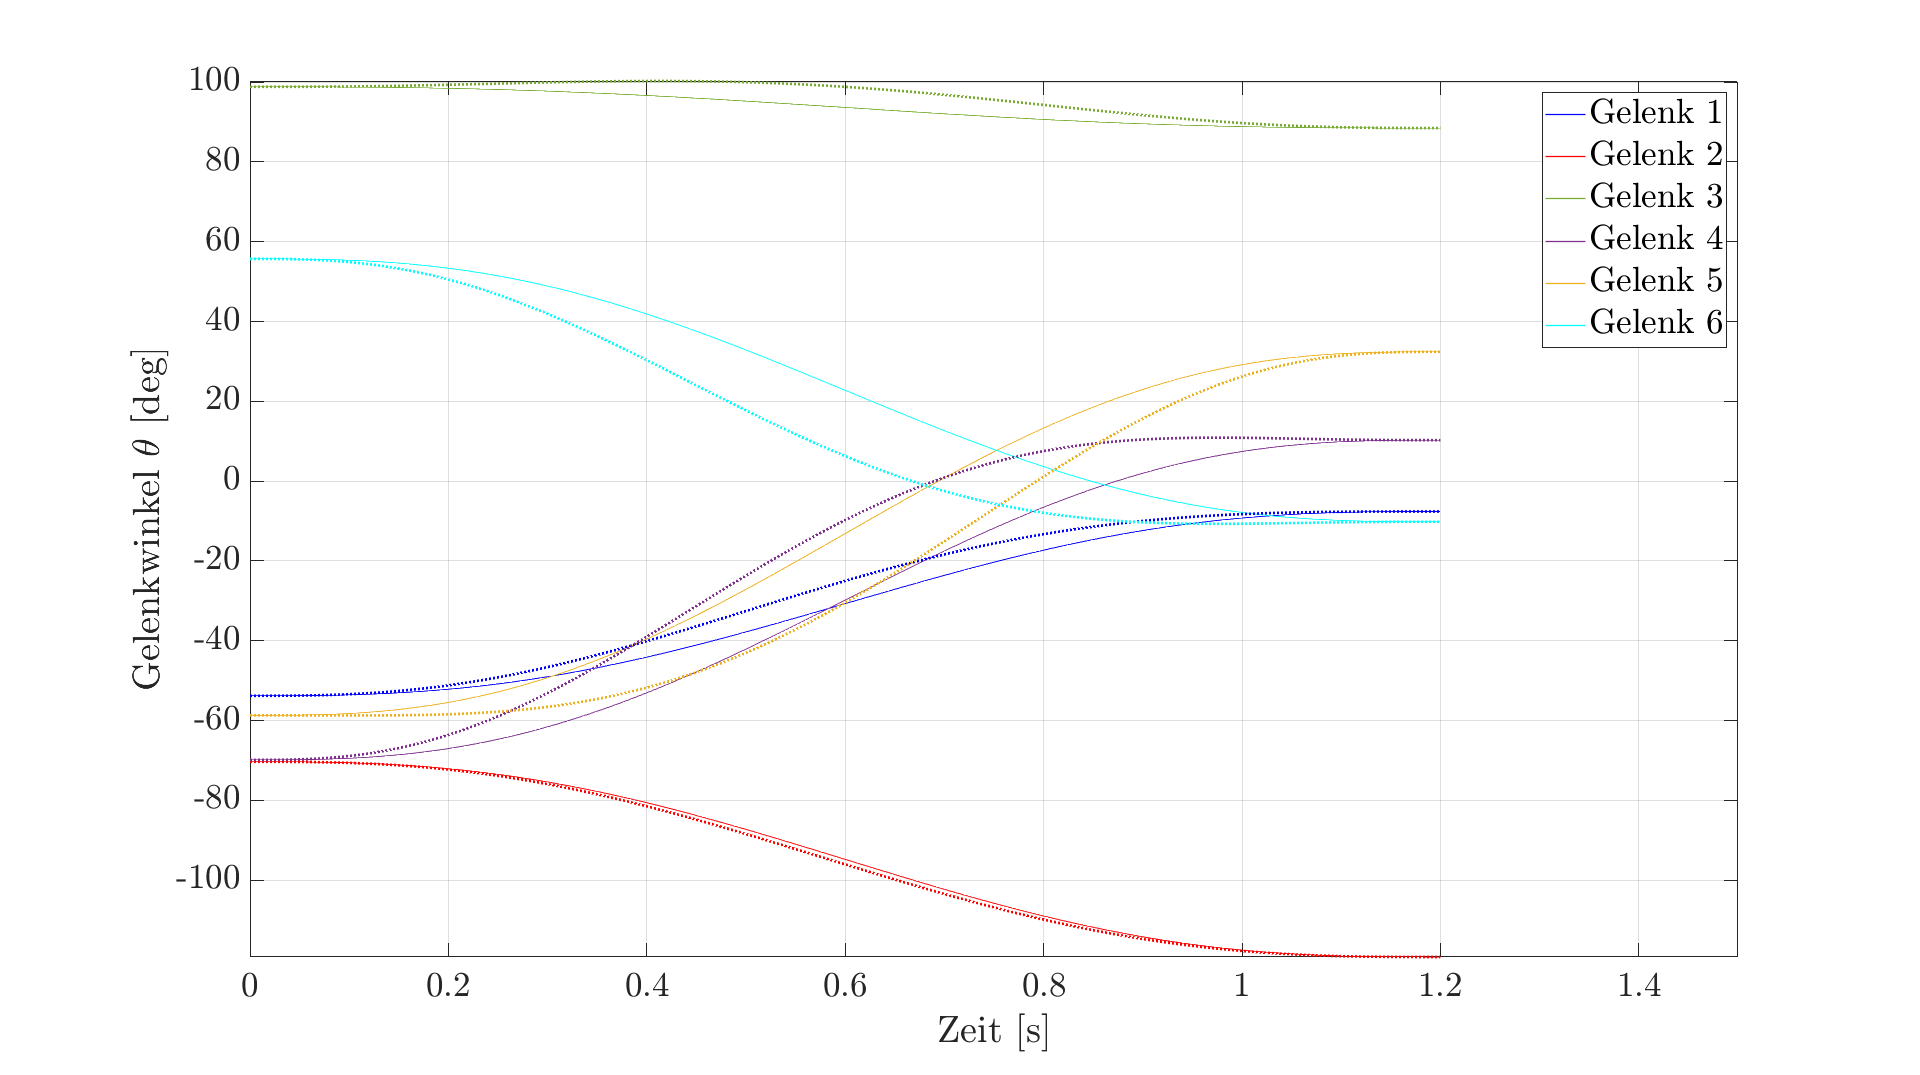
\includegraphics[width=1\linewidth]{images/Optimierungsergebnisse_up/posoptfinal}
	\caption{Simulierte Gelenkwinkel  der Initialbewegung  und justierten, energieoptimierten Bewegungsbahn vom letzten Prozesspunkt auf die  Home Position im Programm Kleben-Seitenwand}
	\label{fig:posoptfinal}
\end{figure}
%
\begin{figure}[tbph]
	\centering
	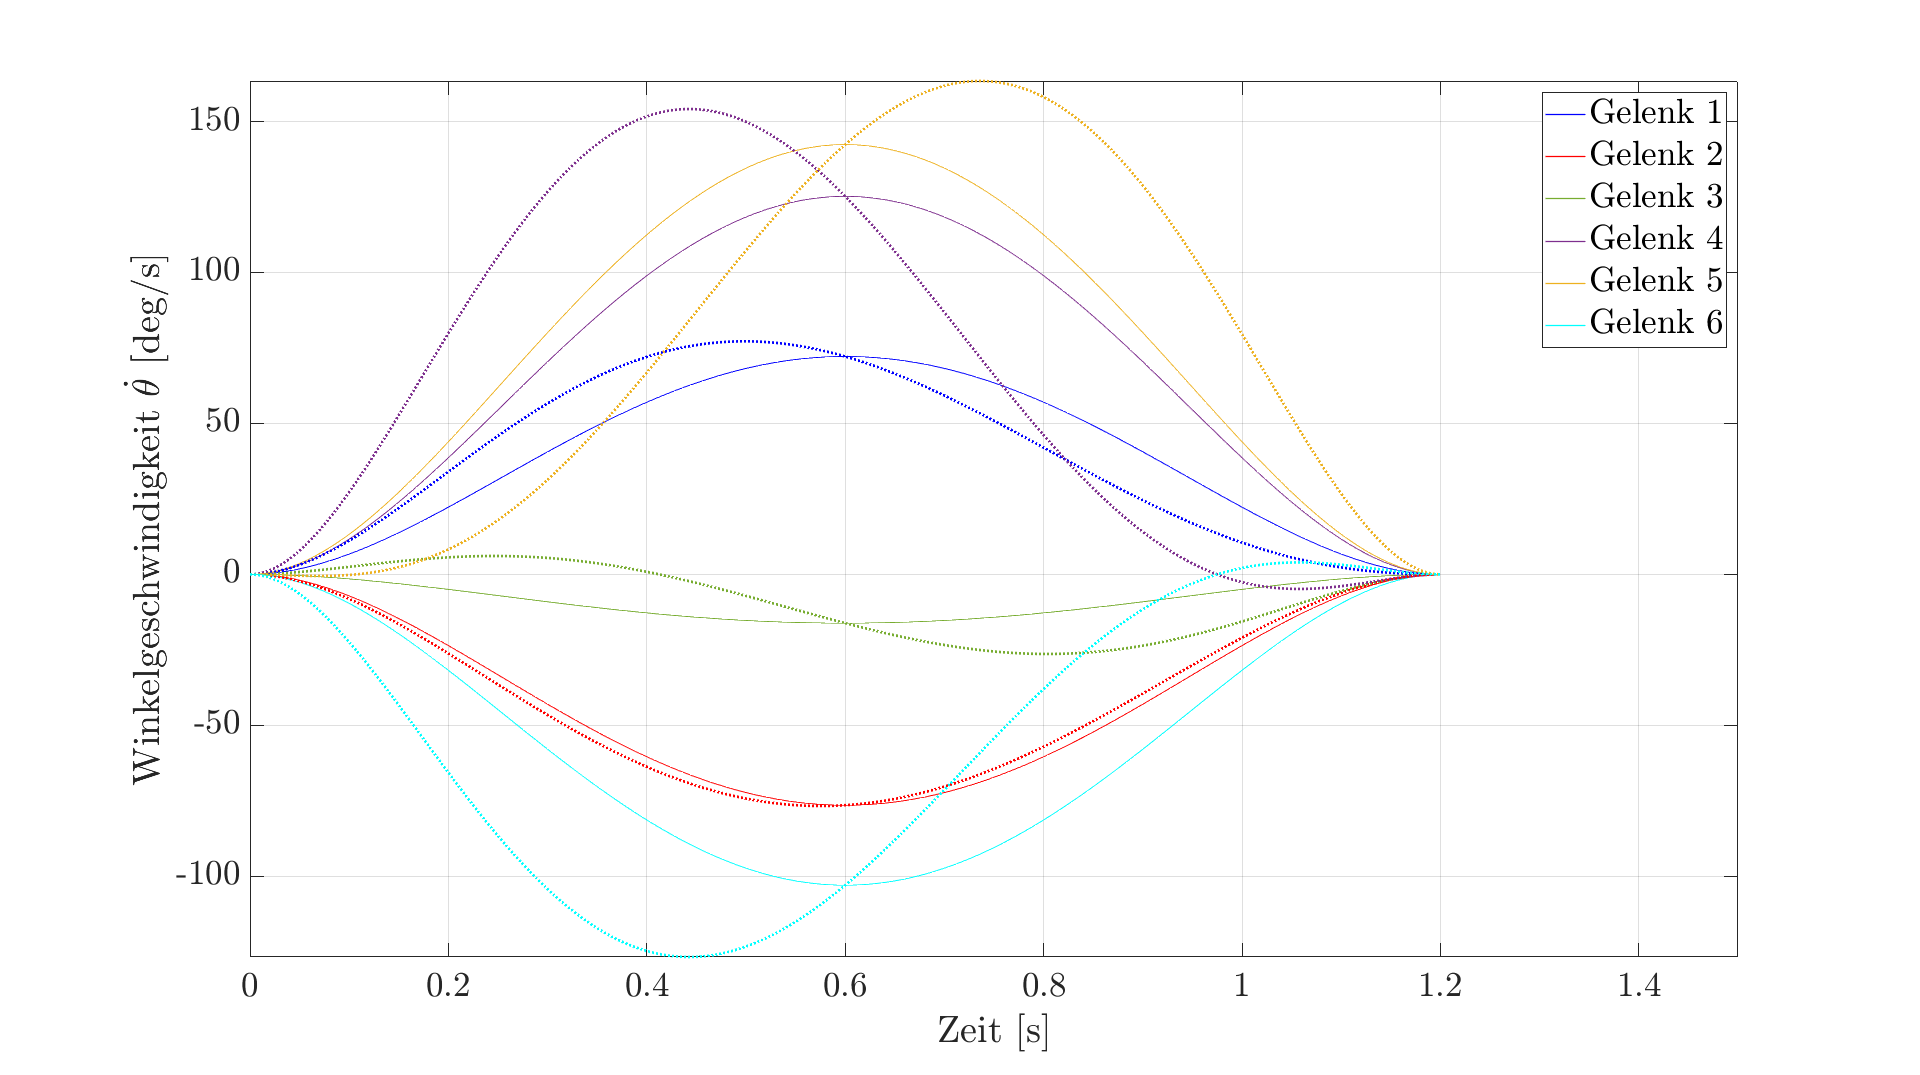
\includegraphics[width=1\linewidth]{images/Optimierungsergebnisse_up/veloptfinal}
	\caption{Simulierte Winkelgeschwindigkeit  der Initialbewegung  und justierten, energieoptimierten Bewegungsbahn vom letzten Prozesspunkt auf die  Home Position im Programm Kleben-Seitenwand}
	\label{fig:veloptfinal}
\end{figure}
%
\begin{figure}[tbph]
	\centering
	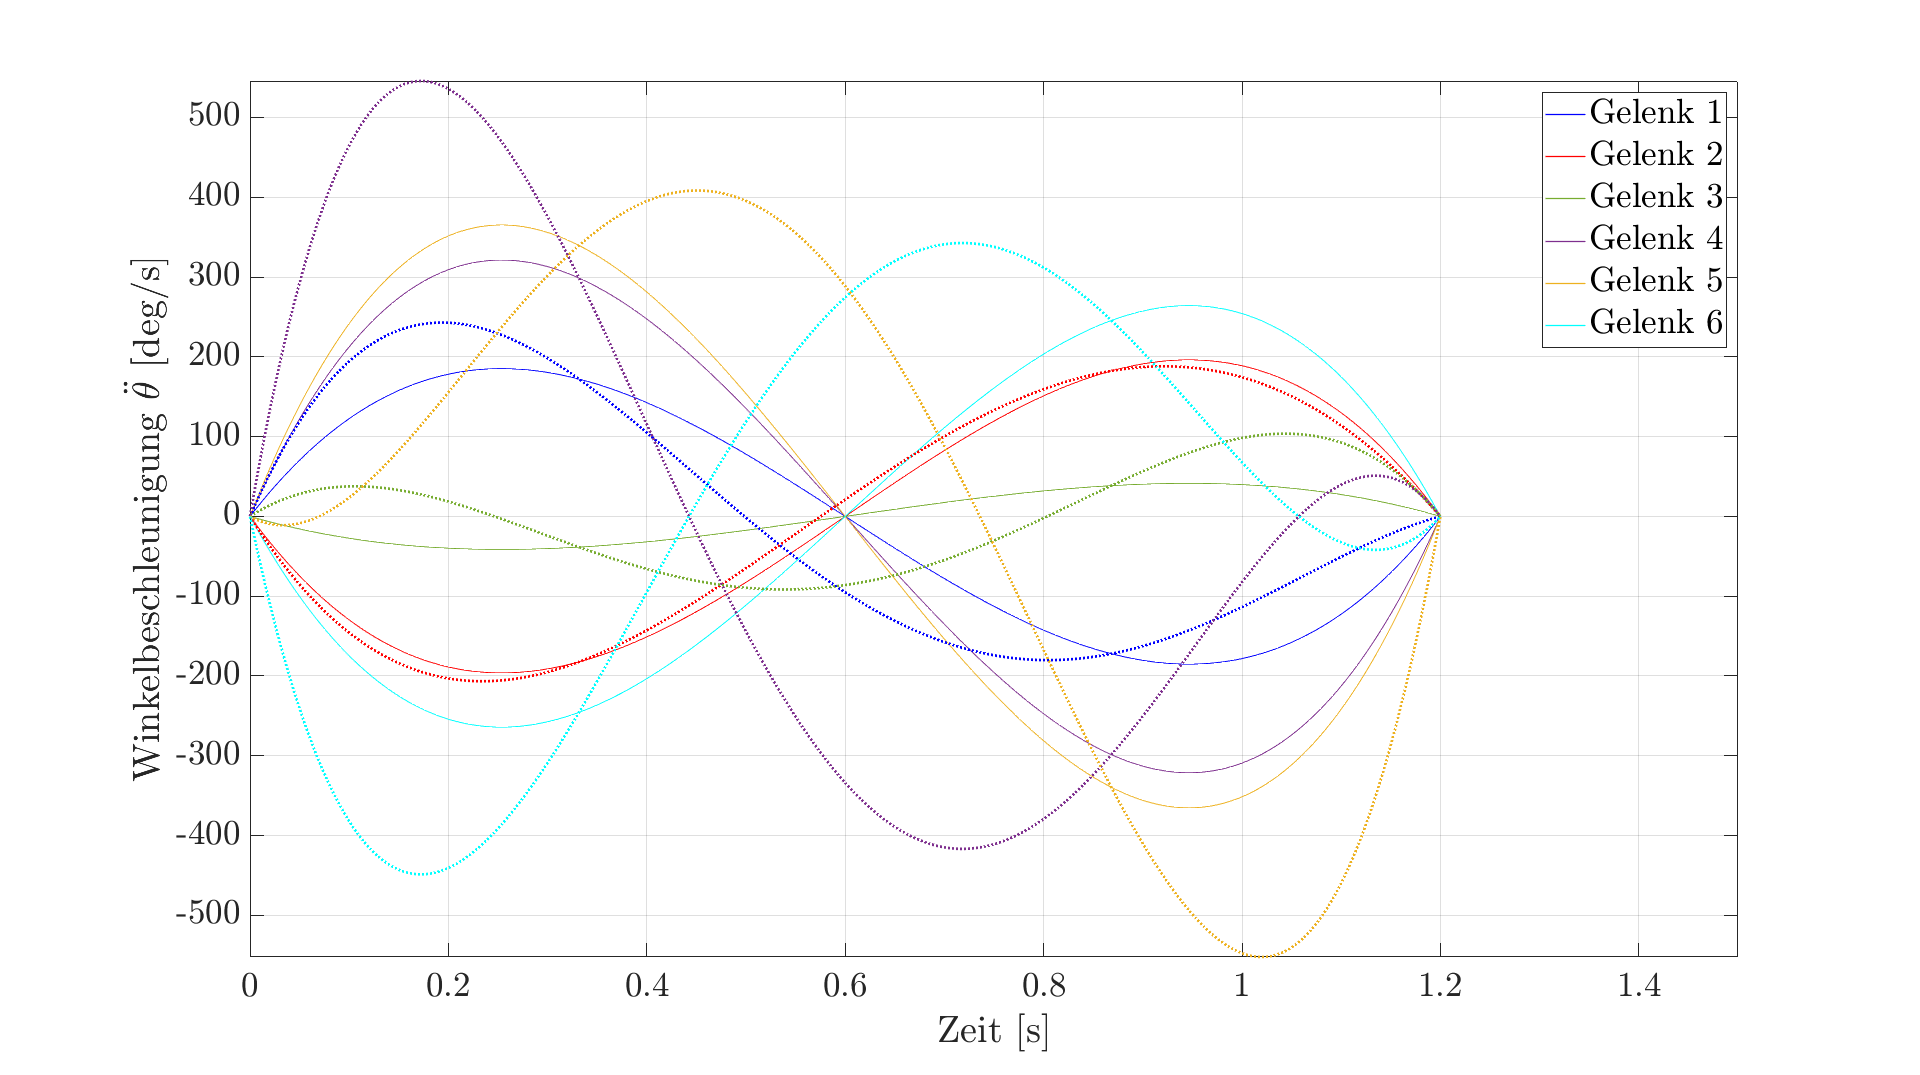
\includegraphics[width=1\linewidth]{images/Optimierungsergebnisse_up/accoptfinal}
	\caption{Simulierte Winkelbeschleunigung  der Initialbewegung  und justierten, energieoptimierten Bewegungsbahn vom letzten Prozesspunkt auf die  Home Position im Programm Kleben-Seitenwand}
	\label{fig:accoptfinal}
\end{figure}
%
%Der qualitative Verlauf der aufgenommenen Drehmomente für den justierten-energieoptimierten Parametervektor entspricht dem des energieoptimierten Parametervektors. 
%
\begin{figure}[tbph]
	\centering
	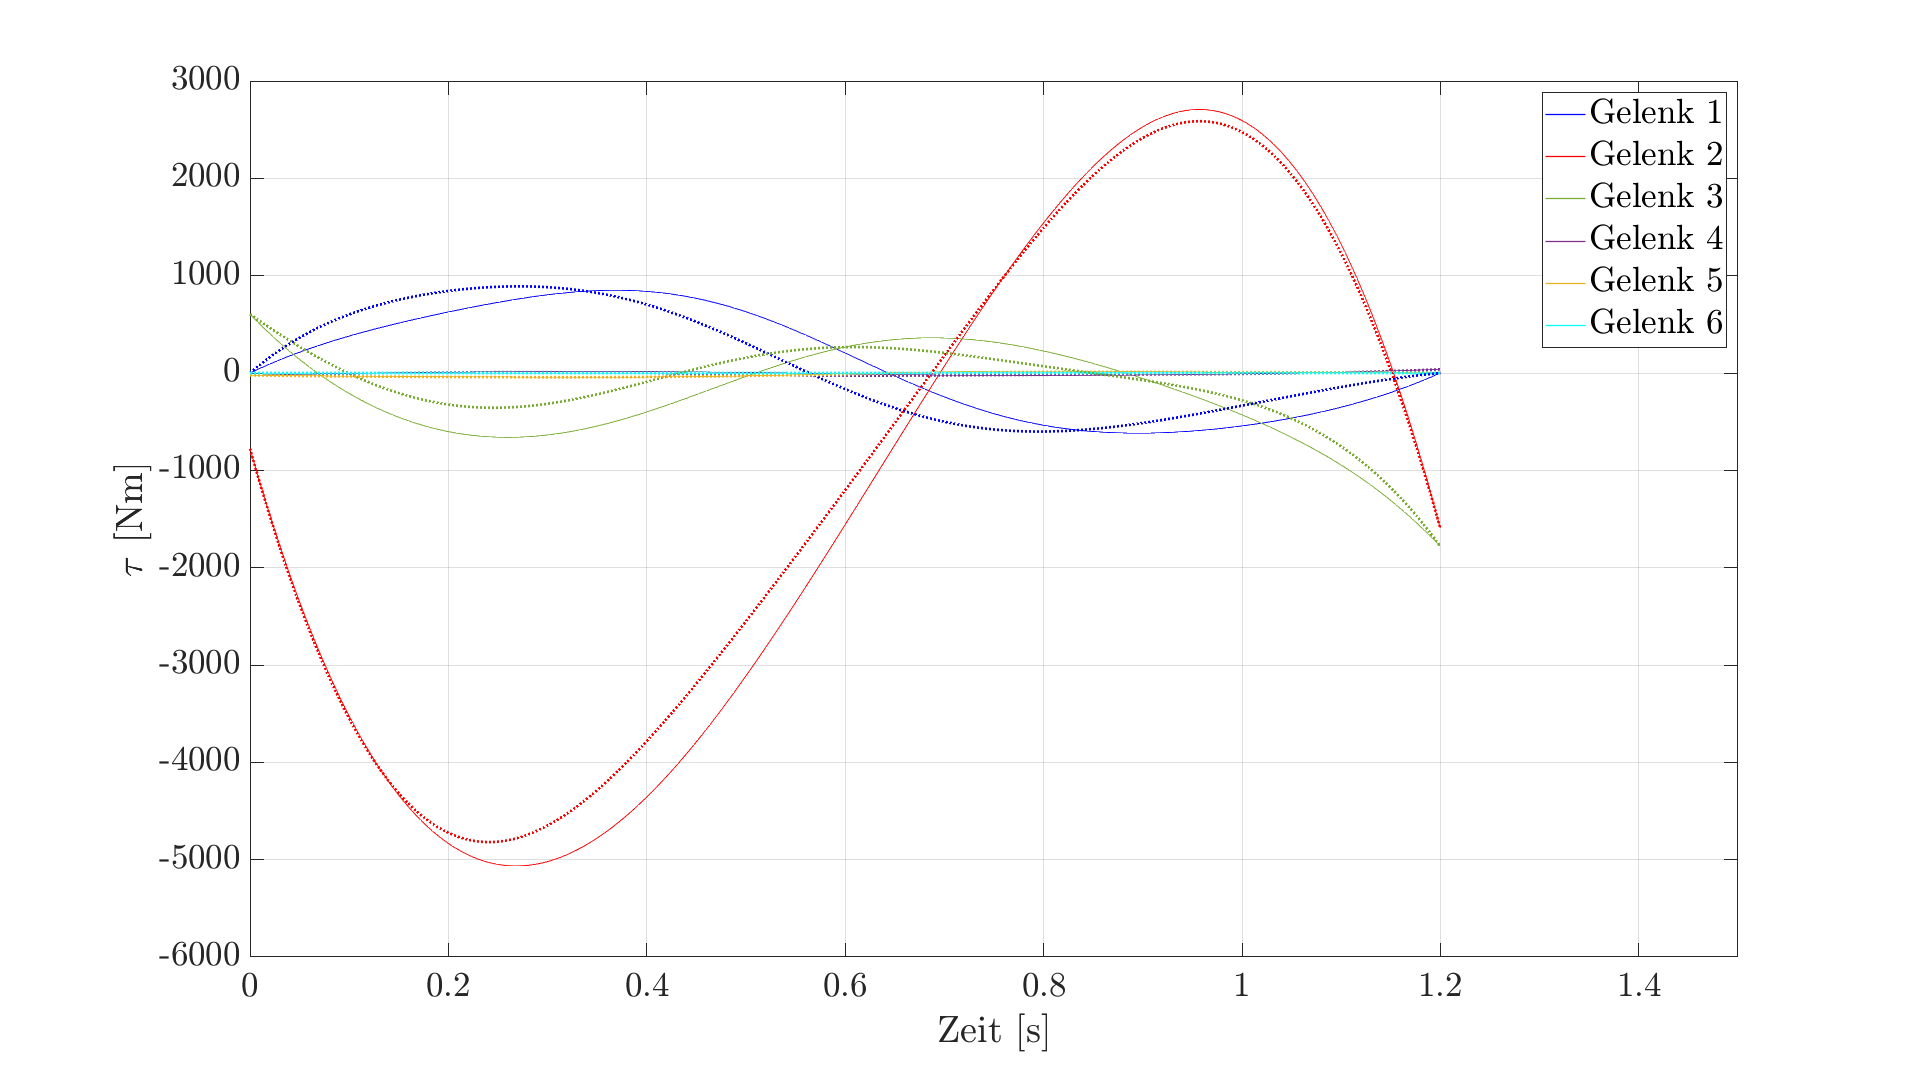
\includegraphics[width=1\linewidth]{images/Optimierungsergebnisse_up/tauoptfinal}
	\caption{Simulierte Drehmomente  der Initialbewegung  und justierten, energieoptimierten Bewegungsbahn vom letzten Prozesspunkt auf die  Home Position im Programm Kleben-Seitenwand}
	\label{fig:tauoptfinal}
\end{figure}
%\begin{figure}[tbph]
%	\centering
%	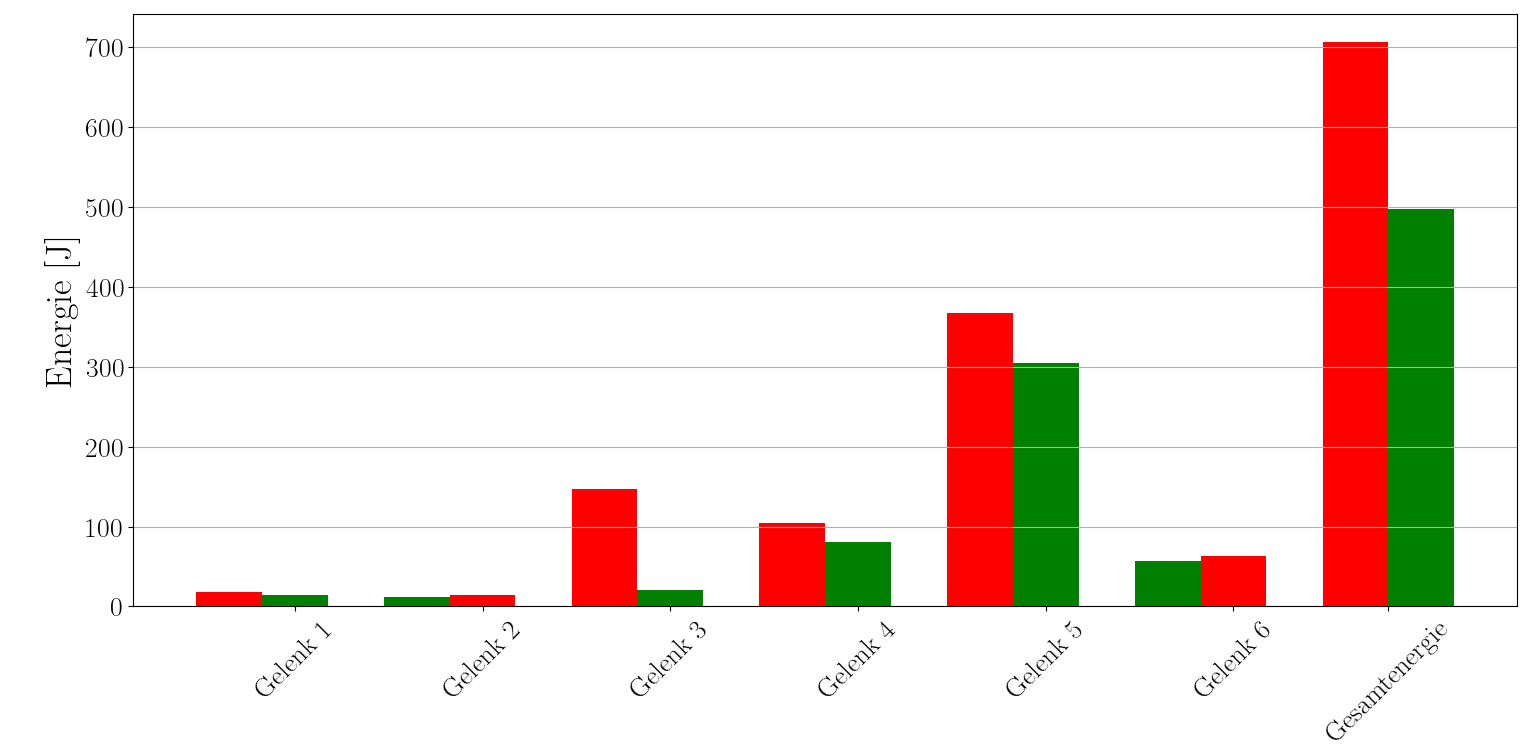
\includegraphics[width=1\linewidth]{images/e_down500}
%	\caption{Energieverbrauch Bewegung Eins}
%	\label{fig:edown500}
%\end{figure}
%\begin{figure}[tbph]
%	\centering
%	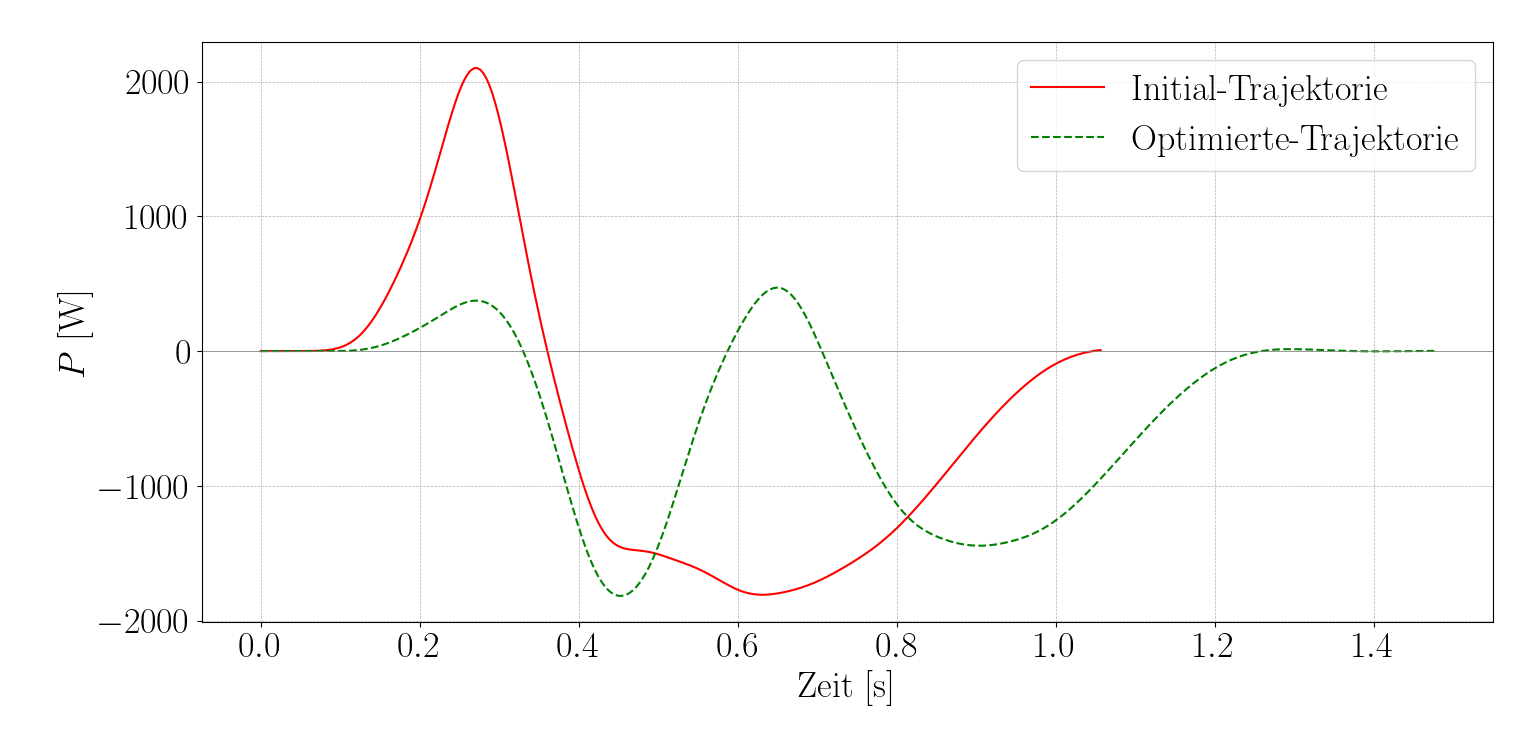
\includegraphics[width=1\linewidth]{images/P_down}
%	\caption{Leistungsaufnahme Bewegung Eins}
%	\label{fig:pdown}
%\end{figure}
%\begin{figure}[tbph]
%	\centering
%	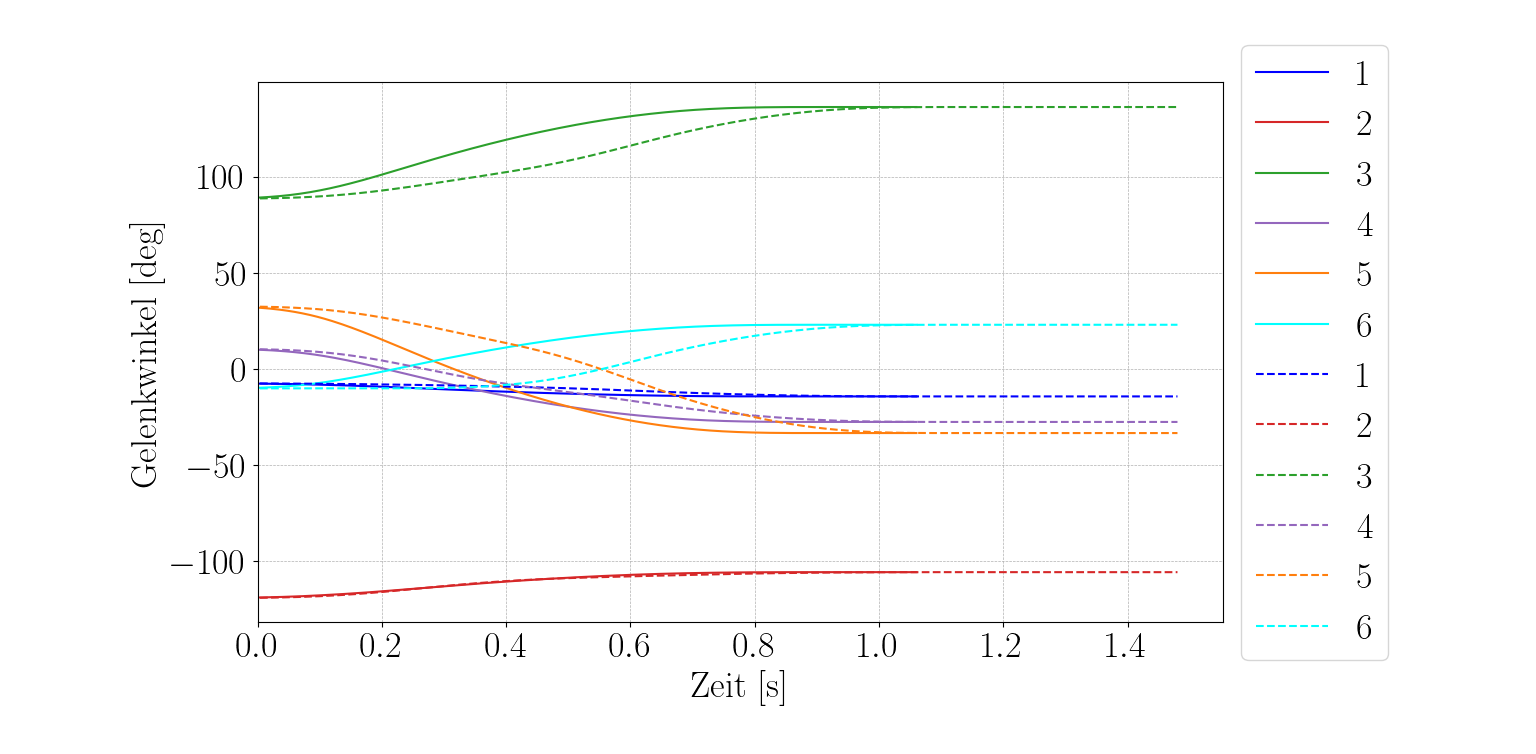
\includegraphics[width=1\linewidth]{images/aiposdown}
%	\caption{Gelenkwinkel Bewegung Eins}
%	\label{fig:aiposdown}
%\end{figure}
%\begin{figure}[tbph]
%	\centering
%	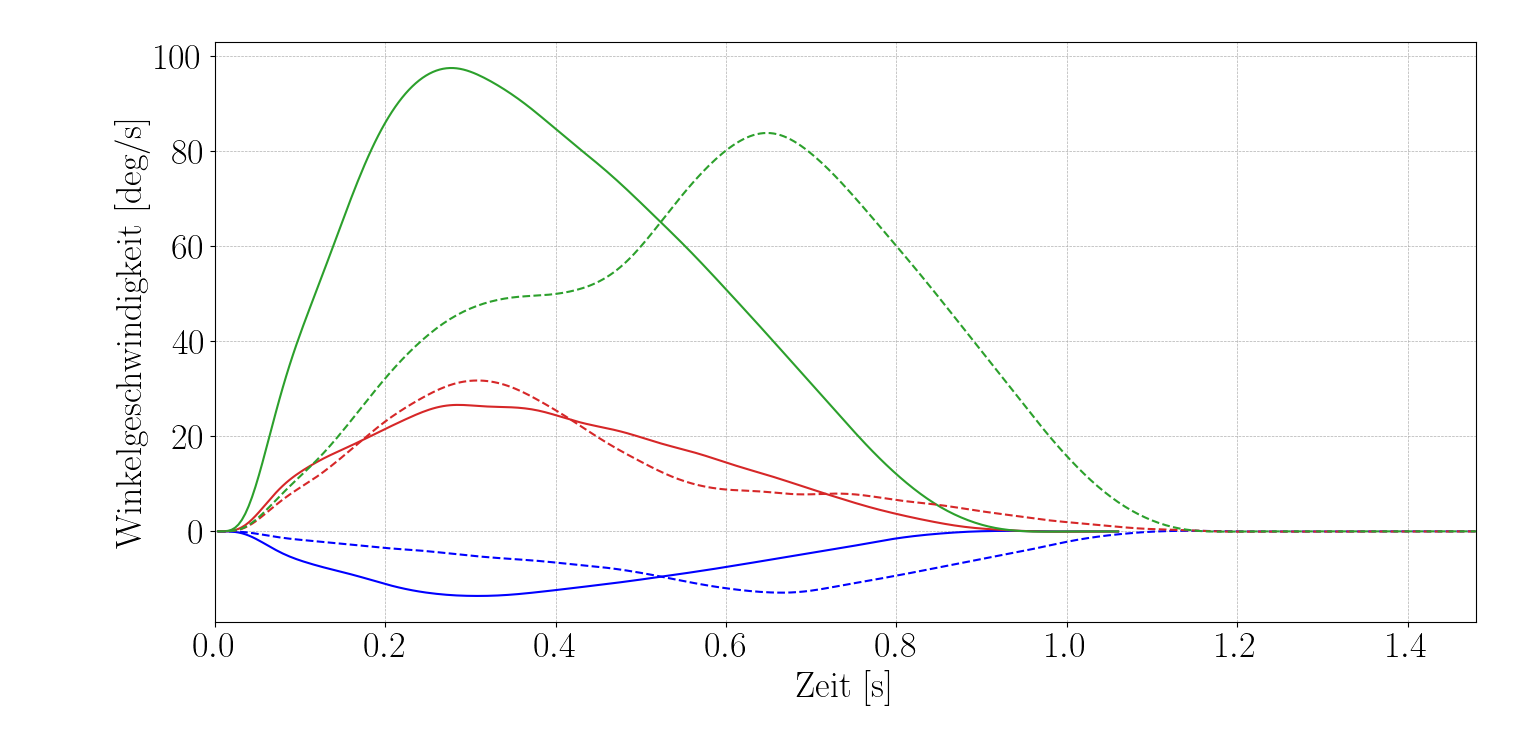
\includegraphics[width=1\linewidth]{images/velposdown1}
%	\caption{Winkelgeschwindigkeit in den Gelenken 1-3 Bewegung Eins}
%	\label{fig:velposdown1}
%\end{figure}
%\begin{figure}[tbph]
%	\centering
%	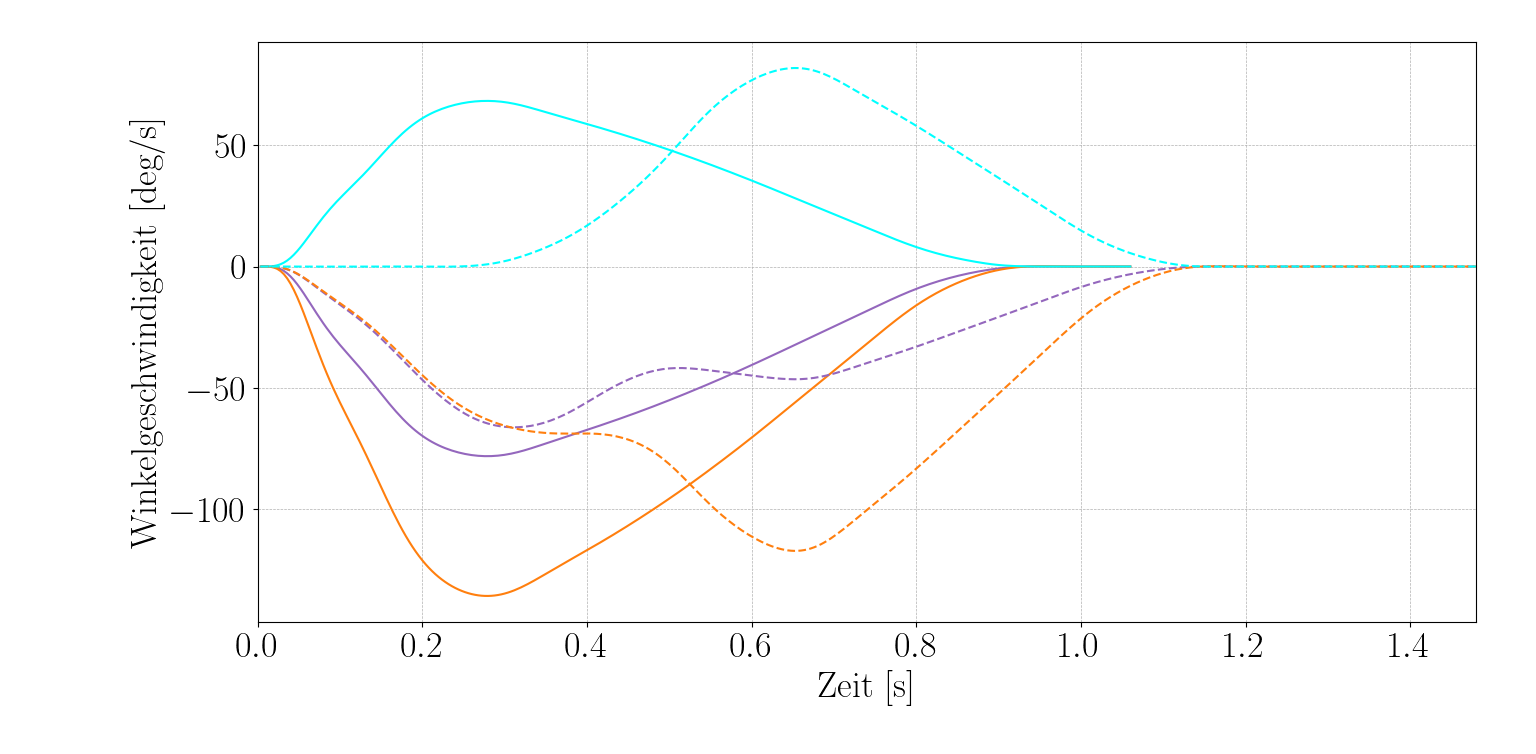
\includegraphics[width=1\linewidth]{images/velposdown2}
%	\caption{Winkelgeschwindigkeit in den Gelenken 4-6 Bewegung Eins}
%	\label{fig:velposdown2}
%\end{figure}
%\begin{figure}[tbph]
%	\centering
%	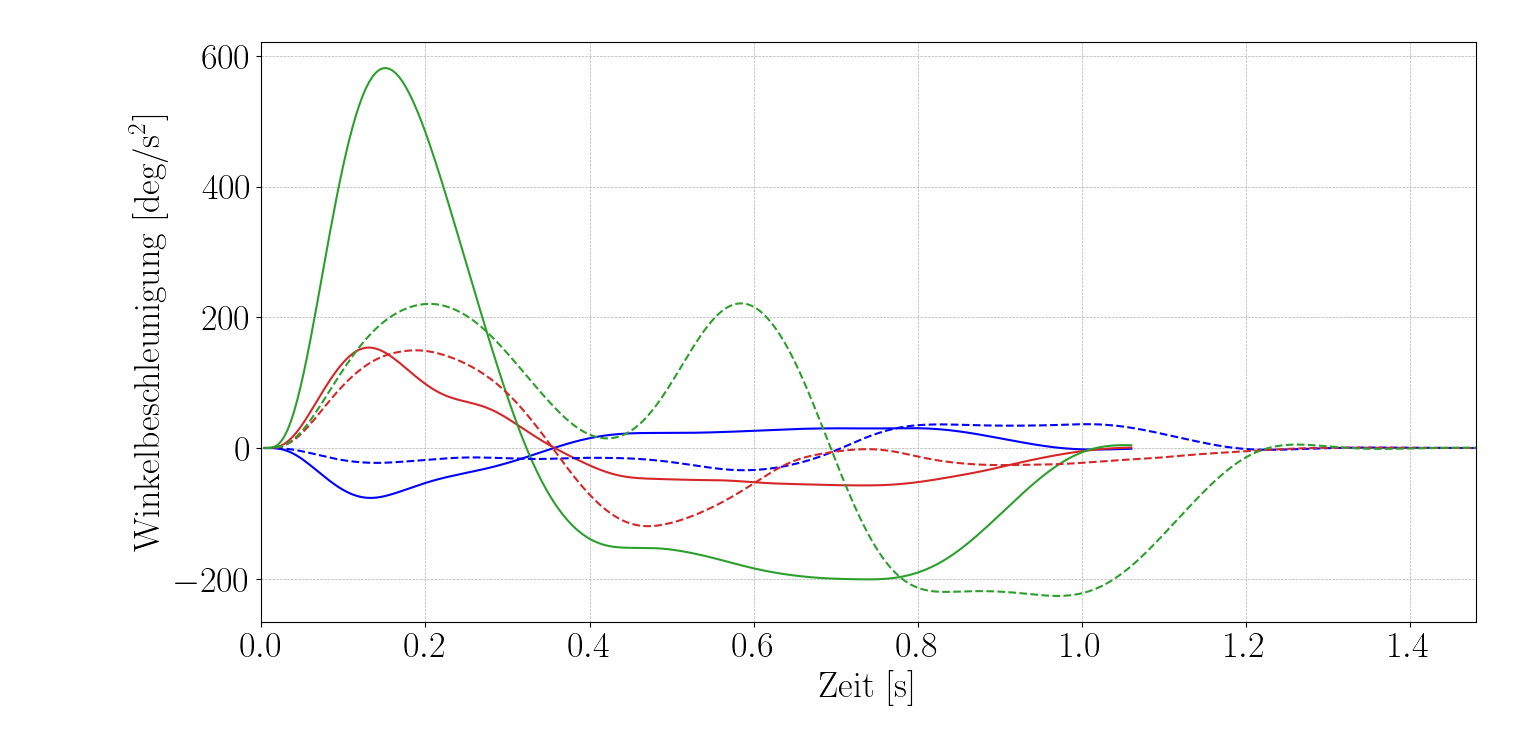
\includegraphics[width=1\linewidth]{images/accdown1}
%	\caption{Winkelbeschleunigung in den Gelenken 1-3 Bewegung Eins}
%	\label{fig:accdown1}
%\end{figure}
%\begin{figure}[tbph]
%	\centering
%	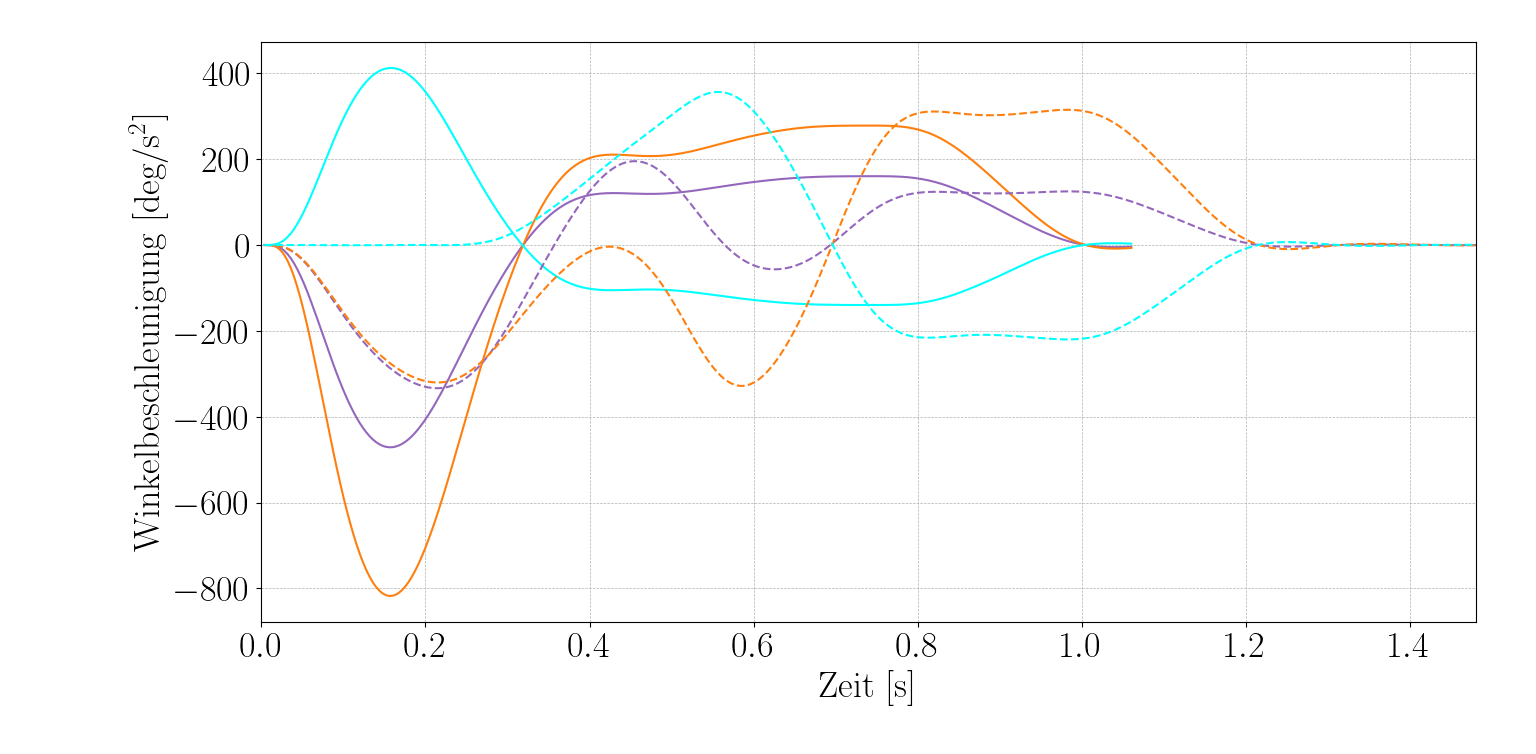
\includegraphics[width=1\linewidth]{images/accdown2}
%	\caption{Winkelbeschleunigung in den Gelenken 4-6 Bewegung Eins}
%	\label{fig:accdown2}
%\end{figure}
%
%\begin{figure}[tbph]
%	\centering
%	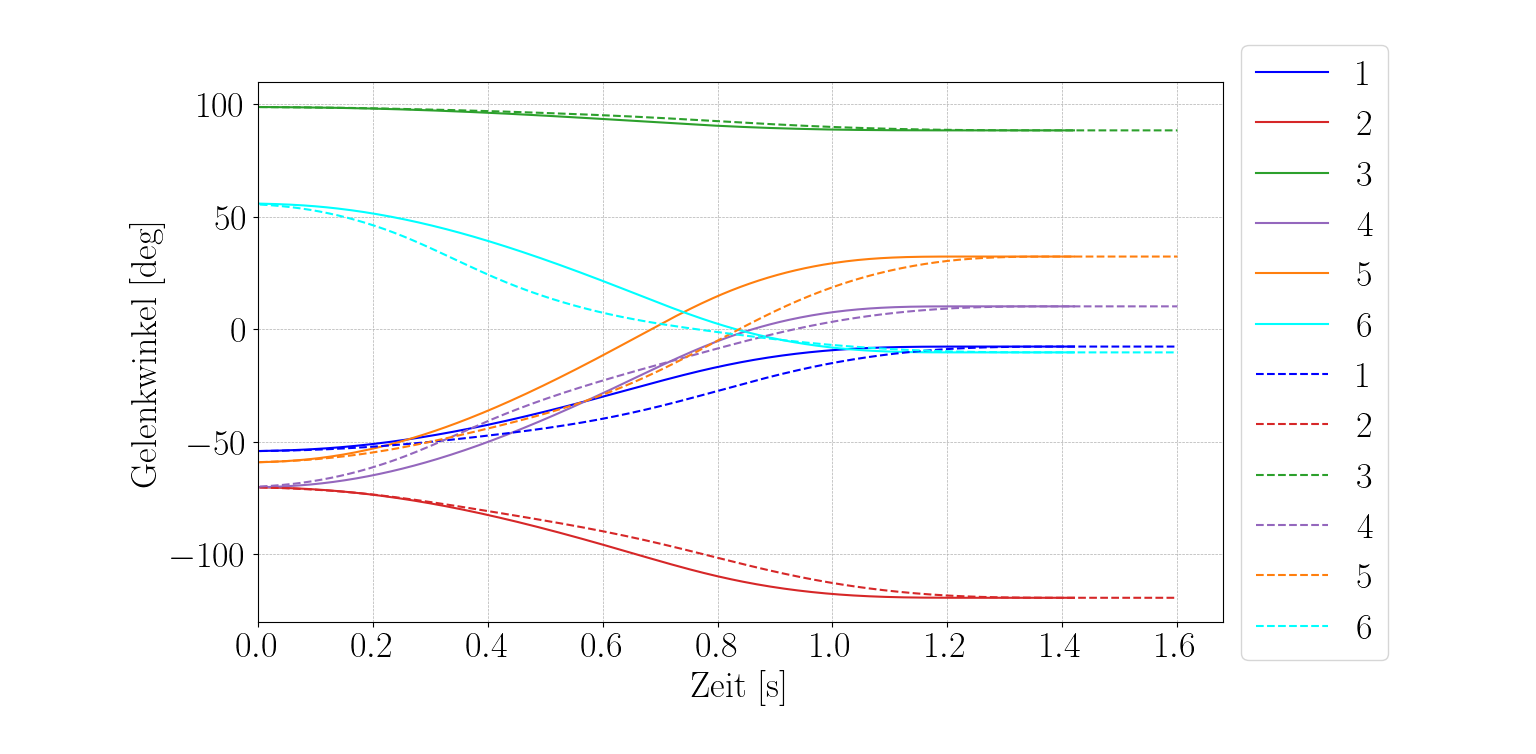
\includegraphics[width=1\linewidth]{images/aiposup}
%	\caption{Gelenkwinkel Bewegung Eins}
%	\label{fig:aiposup}
%\end{figure}
%\begin{figure}[tbph]
%	\centering
%	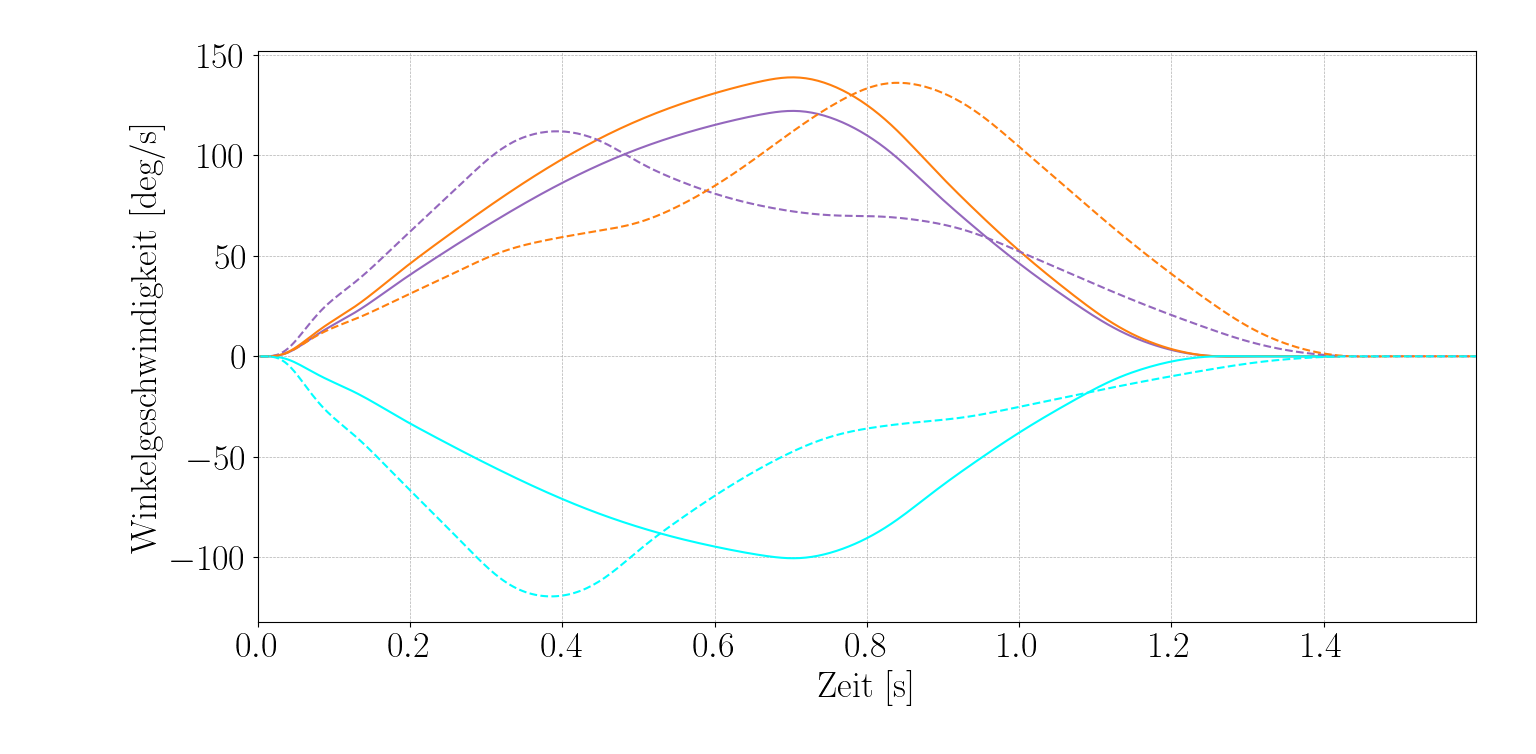
\includegraphics[width=1\linewidth]{images/velposup2}
%	\caption{Winkelgeschwindigkeit in den Gelenken 4-6 Bewegung Zwei}
%	\label{fig:velposup2}
%\end{figure}
%\begin{figure}[tbph]
%	\centering
%	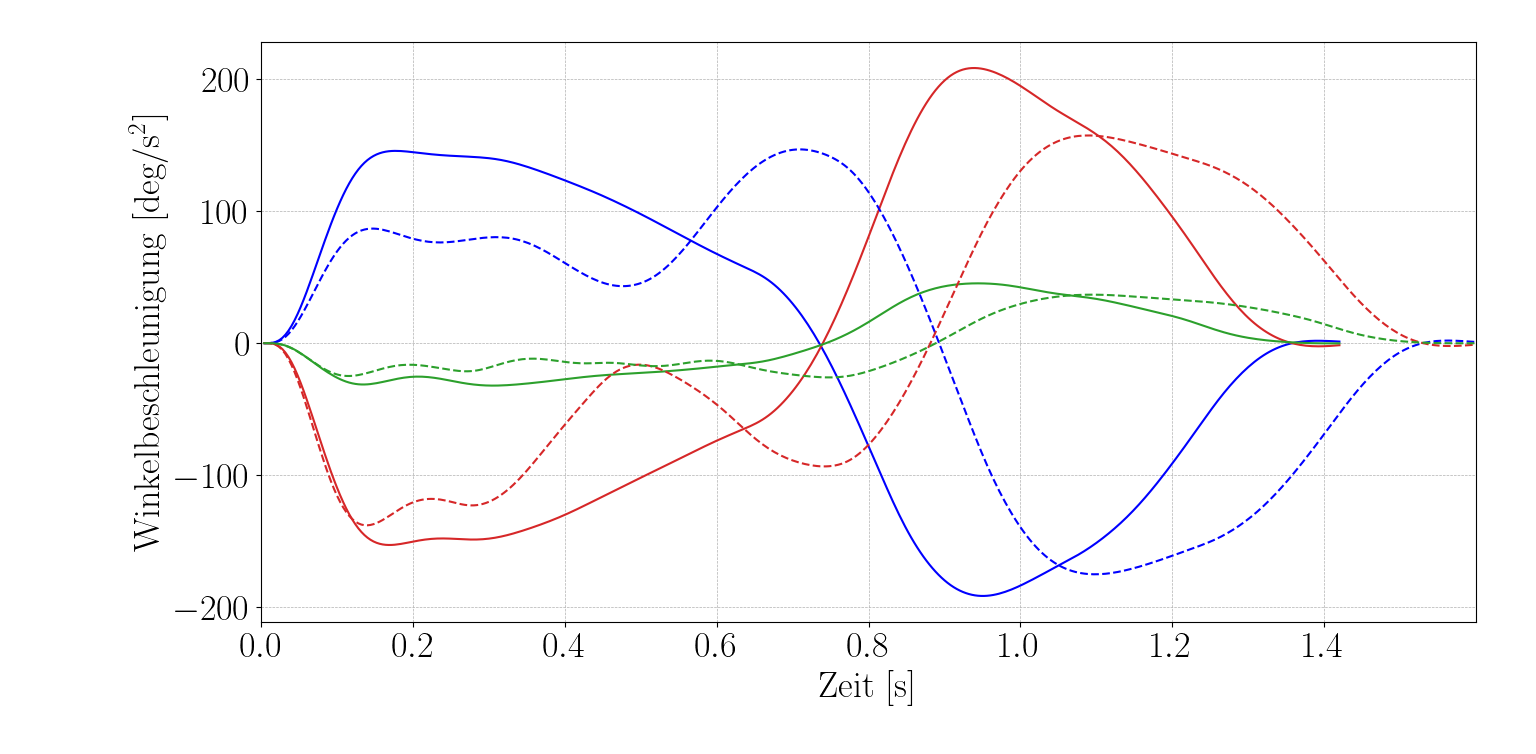
\includegraphics[width=1\linewidth]{images/accup1}
%	\caption{Winkelbeschleunigung in den Gelenken 1-3 Bewegung Zwei}
%	\label{fig:accup1}
%\end{figure}
%\begin{figure}[tbph]
%	\centering
%	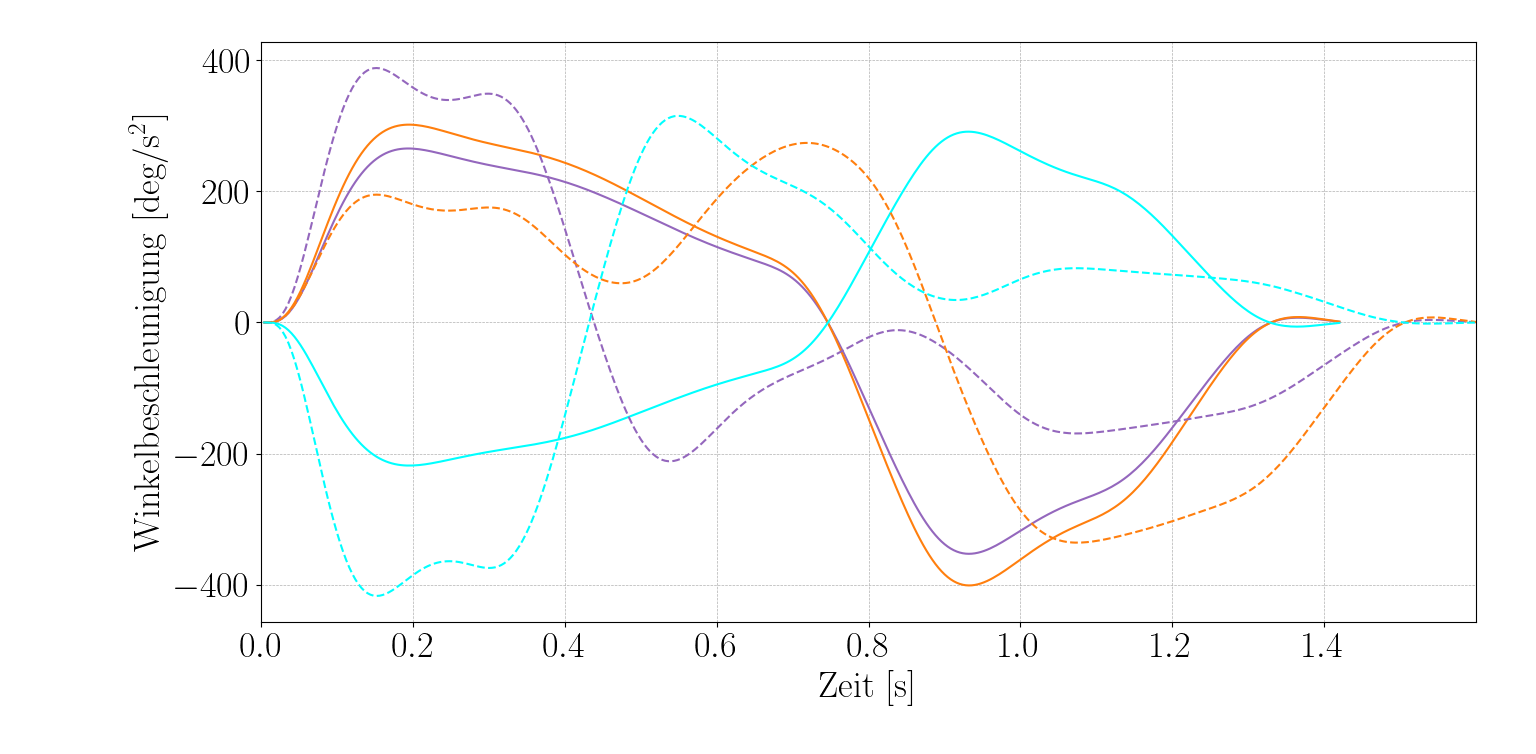
\includegraphics[width=1\linewidth]{images/accup2}
%	\caption{Winkelbeschleunigung in den Gelenken 4-6 Bewegung Zwei}
%	\label{fig:accup2}
%\end{figure}